\chapter{Quantum mechanics in one Dimension}
Material for this chapter can be found in Physics of resonant tunneling. The one-dimensional double-barrier case, B. Ricco and M.Ya. Azbel, Phys. Rev. B 29, 1970 (1984).
Quantum mechanics in one dimension is not only simple, it is also illustrative (many essential situations already arise in dim = 1) and even relevant, the latter especially in relation to the physics of micro- ($\mu m$) and nano-($nm$) structures. In the following, we first deal with the case of pinned constant potentials, cf. Fig. 3.1.
%图 3.1
\begin{figure}[ht]
    \centering
    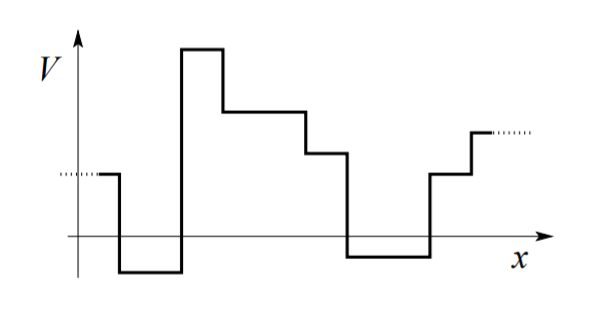
\includegraphics[scale=1]{3_1.PNG}
    \captionsetup{font={Large}}
    \caption{Piecewise constant potential.}
    \label{fig:3_1}
\end{figure}
As special cases we then examine different potentials with exemplary character, in particular bound states in pot (Figure 3.2 (a)), the tunneling effect through a potential barrier (Figure 3.2 (b)), different scattering problems that lead to resonances ( Fig. 3.2 (c) and (d)), the $\delta$-function potential (Fig. 3.2 (e)), periodic potentials leading to energy bands (Fig. 3.2 (f)), or disordered potentials representing the wave function locate (Figure 3.2 (g)).\\\\
\begin{figure}[ht]
    \centering
    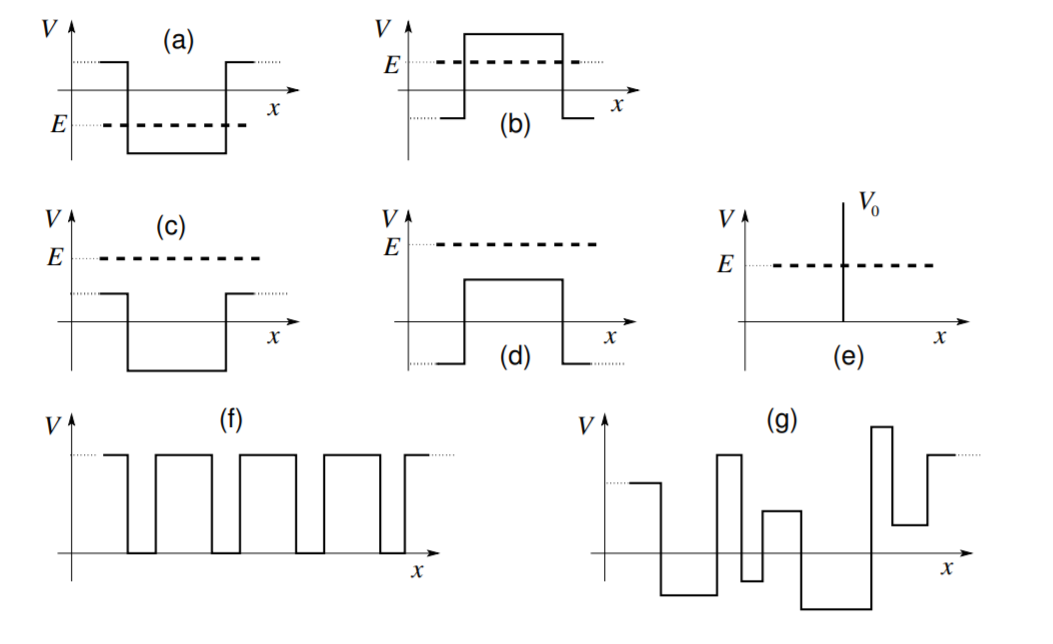
\includegraphics[scale=1]{3_2.PNG}
    \captionsetup{font={Large}}
    \caption{(a) Bonded states in pot, (b) tunneling effect through potential barrier, (b), (c), (d) and (e) scattering problems and resonances, (e) δpotential, (f) periodic potential, (g) random potential.}
    \label{fig:3_2}
\end{figure}
Then we consider some exactly solvable cases, the harmonic oscillator, see Fig. 3.3 (a), the Morse potential, see Fig. 3.3 (b), the $cosh^{-2} x$ potential, see Fig. 3.3 (c) , and the constant force field, cf. Fig. 3.3 (d). In all cases, the Hamiltonian has the form $H = p^2 / 2m + V (x)$, where the potential $V (x)$ takes the form described.
%图 3.3
\begin{figure}[ht]
    \centering
    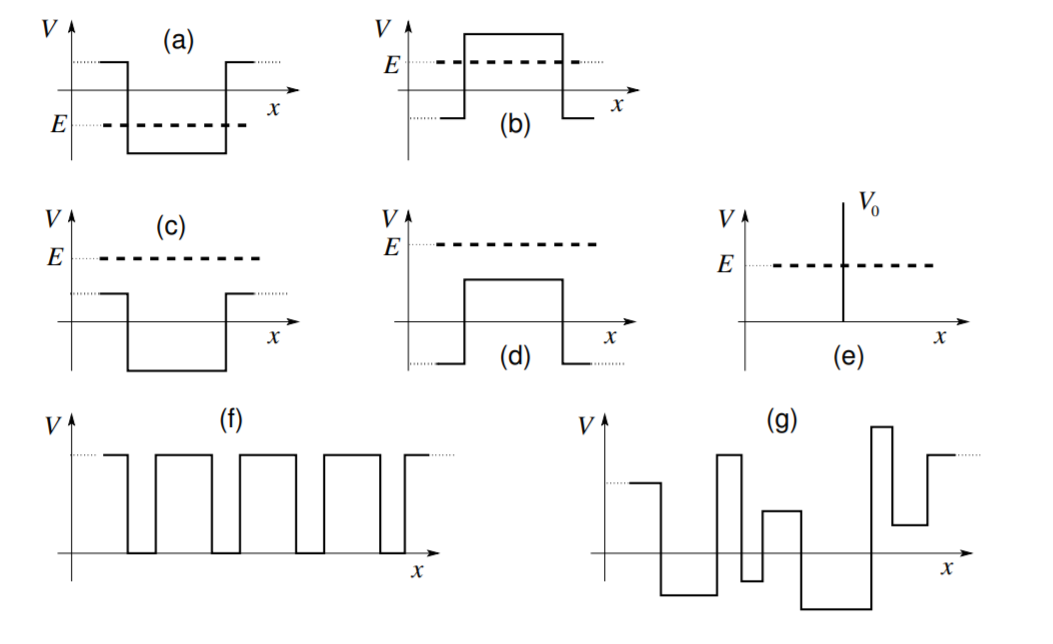
\includegraphics[scale=1]{3_2.PNG}
    \captionsetup{font={Large}}
    \caption{Exactly solvable problems: (a) harmonic potential, (b) the Morse potential that approximates a surface potential, (c) the Cosekans hyperbolic potential (the corresponding eigenvalue problem occurs in different situations), (d) the constant Force field, eg, an electron in the electric field.}
    \label{fig:3_3}
\end{figure}

%Page79
\section{Transfermatrix formalism}
Consider the potential level outlined in Figure 3.4. We are interested in stationary states Ψ which satisfy the time independent equation $H\Psi = E\psi$. The generic solutions to this eigenvalue problem with stuck constant $V$ are $exp \pm ikx)$ if $E> V$ and $exp (\pm αx)$ for $E <V$. Accordingly, we define the wave functions
%图 3.4
\begin{figure}[ht]
    \centering
    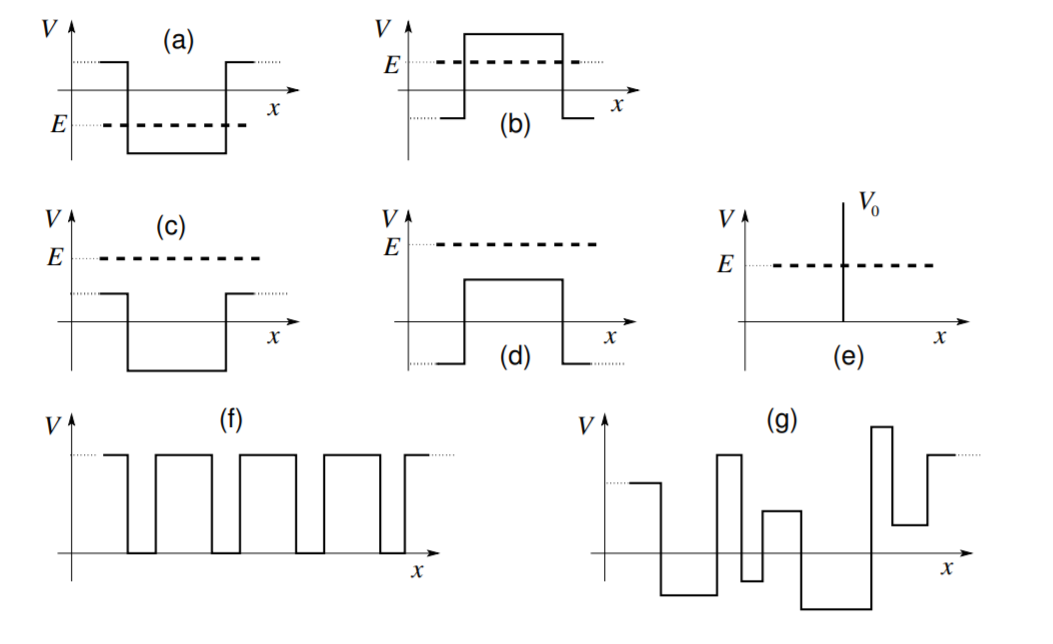
\includegraphics[scale=1]{3_2.PNG}
    \captionsetup{font={Large}}
    \caption{Potential level as element in the transfer matrix
    Formalism.}
    \label{fig:3_4}
\end{figure}
%公式 3.1
\begin{equation}
    \Psi_l=ae^{ikx}+b^{-ikx},\quad \Psi_r=Ae^{-\alpha x}+Be^{\alpha x}
\end{equation}
with
%公式 3.2
\begin{equation}
    k=\sqrt{2mE}/\hbar,\quad \alpha=\sqrt{2m(E_b-E)}/\hbar.
\end{equation}
Stationary states of H must be continuous in $x$ such that $\Psi_l (0) = \Psi_r (0)$ and $\Psi_l^{\prime} (0) = \Psi_r^{\prime} (0)$, where $\prime$ is the usual derivative $\partial x = d / dx$ denotes (otherwise ∂2xin H produces a $\delta$-function in $0$, if in Hamiltonian different (effective) masses $m_l \neq m_r$ the correct hermitian form must be used). The evaluation of the continuity condition connects the amplitudes,
%图 3.5
\begin{figure}[ht]
    \begin{minipage}{0.5\textwidth}
        \centering
        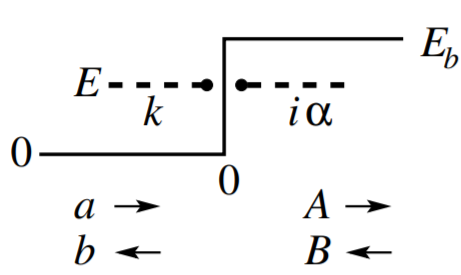
\includegraphics[scale=1]{3_5.PNG}
        \captionsetup{font={Large}}
        \caption{Potential step}
    \end{minipage}
    \begin{minipage}{0.5\textwidth}
        \begin{equation}
            \begin{aligned}
            \left(\begin{array}{cr}{a} 
            \\ {b}\end{array}\right) &=\frac{1}{2}\left(\begin{array}{cc}{1+\frac{i \alpha}{k}} & {1-\frac{i \alpha}{k}} 
            \\ {1-\frac{i \alpha}{k}} & {1+\frac{i \alpha}{k}}\end{array}\right)\left(\begin{array}{c}{A} 
            \\ {B}\end{array}\right) 
            \\ &=M\left(\begin{array}{cc}{A} 
            \\ {B}\end{array}\right), \quad \operatorname{det} M=\frac{i \alpha}{k} &
            \end{aligned}
            \end{equation}
            
            \begin{equation}
                \begin{aligned}
                \left(\begin{array}{cr}{A} 
                \\ {B}\end{array}\right) &=\frac{1}{2}\left(\begin{array}{cc}{1+\frac{k}{i \alpha}} & {1-\frac{k}{i \alpha}} 
                \\ {1-\frac{k}{i \alpha}} & {1+\frac{k}{i \alpha}}\end{array}\right)
                \left(\begin{array}{c}{a} 
                \\ {b}\end{array}\right) 
                \\ &=M^{-1}\left(\begin{array}{cc}{a} 
                \\ {b}\end{array}\right), \quad \operatorname{det} M^{-1}=\frac{k}{i \alpha} &
                \end{aligned}
                \end{equation}
    \end{minipage}

\end{figure}
%公式 3.3
%公式 3.4
%Page80
Likewise, we obtain the transfer matrix (using the approach $Ψ_l = ae^{-αx} + be^{αx}$ and $Ψ_r = Ae^{ikx} + Be^{-ikx}$)for the inverse step
图 3
%公式 3.5
\begin{figure}[ht]
    \begin{minipage}{0.5\textwidth}
        \centering
        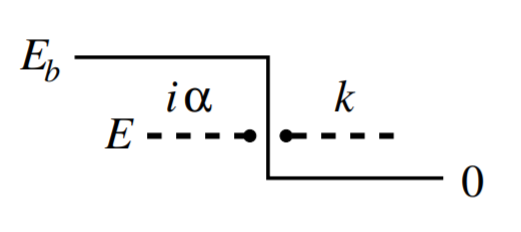
\includegraphics[scale=1]{3_5_1.PNG}
    \end{minipage}
    \begin{minipage}{0.5\textwidth}
        \begin{equation}
            \begin{aligned}
                M = &\frac{1}{2}\left(\begin{array}{cc}{1+\frac{k}{i \alpha}} & {1-\frac{k}{i\alpha}}\\{1-\frac{k}{i\alpha}}&{1+\frac{k}{i\alpha}}
                \end{array}\right),
                \\& \operatorname{det}M=\frac{k}{i\alpha},
            \end{aligned}
        \end{equation}
    \end{minipage}
\end{figure}
and further:\\
%公式 3.6
\begin{figure}[ht]
    \begin{minipage}{0.5\textwidth}
        \centering
        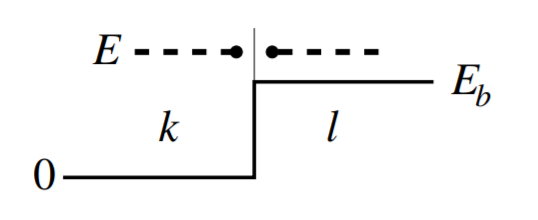
\includegraphics[scale=1]{3_5_2.PNG}
    \end{minipage}
    \begin{minipage}{0.5\textwidth}
        \begin{equation}
            \begin{aligned}
                M = &\frac{1}{2}\left(\begin{array}{cc}{1+\frac{l}{k}} & {1-\frac{l}{k}}\\{1-\frac{l}{k}}&{1+\frac{l}{k}}
                \end{array}\right),
                \\l =& \sqrt{2m(E-E_b)}/\hbar<k,
            \end{aligned}
        \end{equation}
    \end{minipage}
\end{figure}

%公式 3.7
\begin{figure}[ht]
    \begin{minipage}{0.5\textwidth}
        \centering
        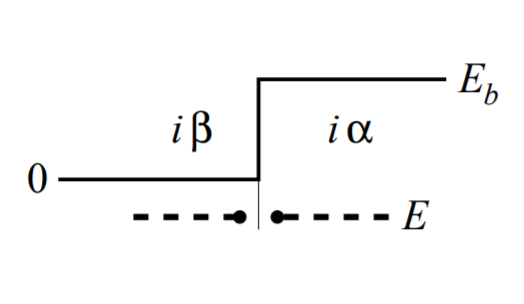
\includegraphics[scale=1]{3_5_3.PNG}
    \end{minipage}
    \begin{minipage}{0.5\textwidth}
        \begin{equation}
            \begin{aligned}
                M = &\frac{1}{2}\left(\begin{array}{cc}{1+\frac{k}{l}} & {1-\frac{k}{l}}\\{1-\frac{k}{l}}&{1+\frac{k}{l}}
                \end{array}\right),
                \\& \operatorname{det}M=\frac{k}{l},
            \end{aligned}
        \end{equation}
    \end{minipage}
\end{figure}

%公式 3.8
\begin{figure}[ht]
    \begin{minipage}{0.5\textwidth}
        \centering
        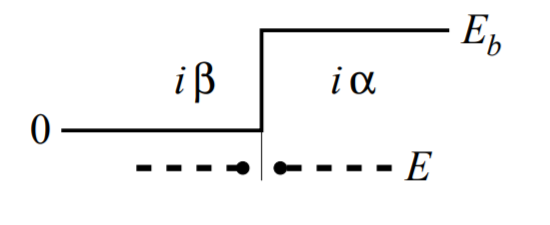
\includegraphics[scale=1]{3_5_4.PNG}
    \end{minipage}
    \begin{minipage}{0.5\textwidth}
        \begin{equation}
            \begin{aligned}
                M = &\frac{1}{2}\left(\begin{array}{cc}{1+\frac{\alpha}{\beta}} & {1-\frac{\alpha}{\beta}}\\{1-\frac{\alpha}{\beta}}&{1+\frac{\alpha}{\beta}}
                \end{array}\right),
                \\\beta =& \sqrt{2m(-E)}/\hbar<\alpha,
            \end{aligned}
        \end{equation}
    \end{minipage}
\end{figure}
%公式 3.9
\begin{figure}[ht]
    \begin{minipage}{0.5\textwidth}
        \centering
        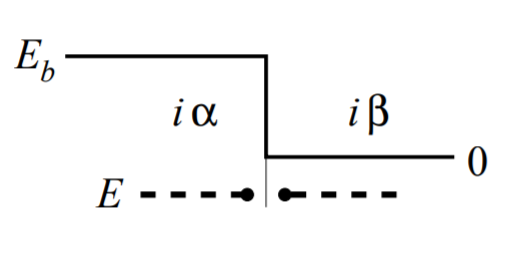
\includegraphics[scale=1]{3_5_5.PNG}
    \end{minipage}
    \begin{minipage}{0.5\textwidth}
        \begin{equation}
            \begin{aligned}
                M = &\frac{1}{2}\left(\begin{array}{cc}{1+\frac{\beta}{\alpha}} & {1-\frac{\beta}{\alpha}}\\{1-\frac{\beta}{\alpha}}&{1+\frac{\beta}{\alpha}}
                \end{array}\right),
                \\& \operatorname{det}M=\frac{\beta}{\alpha},
            \end{aligned}
        \end{equation}
    \end{minipage}
\end{figure}
In addition, we need matrices, which are the 'propagation' over and over again describe constant potentials. For positive energies take legal and left-hander the phases $exp (ikw)$ and $exp (-ikw)$, where w denotes the propagation distance; in the area of ​​forbidden propagation, the waves are damped, $\Psi^{\to}_r = e^{-αw}Ψ^{\to}_l$ for right-wing and $\Psi^{\leftarrow}_l = e^{-αw}Ψ^{\gets}_r$ for left-handers, where $r$ and $l$ are the right and left ends of the left Interval (see sketch) and the arrows $\to$ or $\gets$ specify the directions. Furthermore, right and left runners do not mix, which results in the transfer matrices.\\
%图
%公式 3.10
\begin{figure}[ht]
    \begin{minipage}{0.5\textwidth}
        \centering
        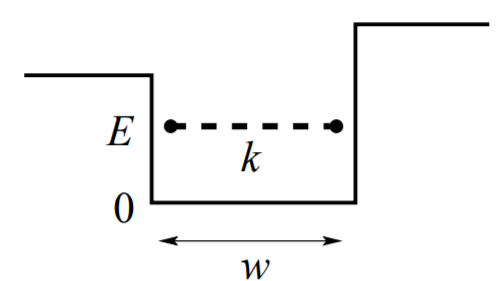
\includegraphics[scale=1]{3_5_6.PNG}
    \end{minipage}
    \begin{minipage}{0.5\textwidth}
        \begin{equation}
            \begin{aligned}
                \widetilde{M} = &\frac{1}{2}\left(\begin{array}{cc}{e^{-ikw}} & {0}\\{0}&{e^{ikw}}
                \end{array}\right),
                \\& \operatorname{det}\widetilde{M}=1,
            \end{aligned}
        \end{equation}
    \end{minipage}
\end{figure}

%公式 3.11
\begin{figure}[ht]
    \begin{minipage}{0.5\textwidth}
        \centering
        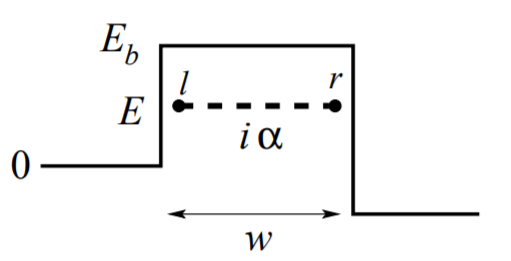
\includegraphics[scale=1]{3_5_7.PNG}
    \end{minipage}
    \begin{minipage}{0.5\textwidth}
        \begin{equation}
            \begin{aligned}
                \widetilde{M} = &\frac{1}{2}\left(\begin{array}{cc}{e^{\alpha w}} & {0}\\{0}&{e^{-\alpha w}}
                \end{array}\right),
                \\& \operatorname{det}\widetilde{M}=1,
            \end{aligned}
        \end{equation}
    \end{minipage}
\end{figure}
The whole problem with stuck wise constant potentials
%图 3.6
\begin{figure}[ht]
    \centering
    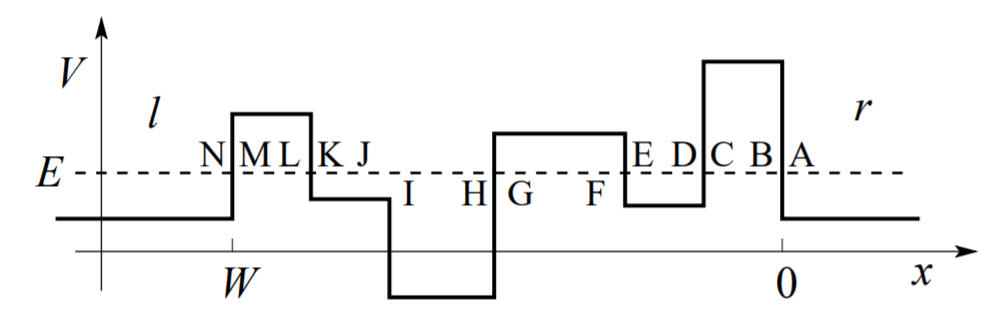
\includegraphics[scale=1]{3_6.PNG}
    \captionsetup{font={Large}}
    \caption{Piecewise constant potential with arbitrary shape.}
\end{figure}
is solved by a simple matrix multiplication; Let the wave function on the right side be given by
%公式 3.12
\begin{equation}
\Psi_r=\left(\begin{array}{cc}{A}\\{B}\end{array}\right),
\end{equation}
then the wave function $Ψ_l$ on the left side results as
%公式 3.13
\begin{equation}
    \begin{aligned}
        \Psi_l = \left(\begin{array}{cc}
            {a}\\{b}
        \end{array}\right)=&M_{NM}\widetilde{M}_{ML}M_{LK}\widetilde{M}_{KJ}M_{JI}\widetilde{M}_{IH}M_{HG}\\
        &\times \widetilde{M}_{GF}M_{FE}\widetilde{M}_{ED}M_{DC}\widetilde{M}_{CB}M_{BA}\left(\begin{array}{cc}
            {A}\\{B}
        \end{array}\right).
    \end{aligned}
\end{equation}

%Page82
Note that the wave functions $Ψ_l$ and $Ψ_r$ are given by
%3.14
\begin{equation}
    \begin{split}
        &\Psi_r = Ae^{ikx}+Be^{-ikx}\\
        &\Psi_l = ae^{ik(x-W)}+be^{-ik(x-W)},\quad (here, W<0)
    \end{split}
\end{equation}
since the matrices $M$ were always referenced to $x = 0$. Of course, the relevant $\alpha, \beta, k, l$ and propagation distances $w$ are always to be used. The above formalism is particularly suitable for numerical solutions (by computer). Since the complete information is always calculated, the solution of specific questions (with some coefficients A$, B, a, b = 0$) is often simpler by means of direct analysis instead of transfer matrix technique.

\section{Scatter Matrix}
An important quantity related to the transfer matrix $M$ is the scattering matrix $S$: Whilst the transfer matrix has the amplitudes $A, B,\cdots $ on the right side of the potential with the amplitudes $a, b,\cdots$ to the left of the potential, the scattering matrix connects the incident amplitudes (e.g., $a$ and $B$) with the falling out amplitudes (e.g., $A$ and $b$),
%公式 3.15
\begin{equation}
\begin{aligned} 
\Psi_{\mathrm{out}}=&\quad
    \left(\begin{array}{c}{b} \\ {A}\end{array}\right) &=\left(\begin{array}{cc}{r} & {t^{\prime}} \\ {t} & {r^{\prime}}\end{array}\right)\left(\begin{array}{c}{a} \\ {B}\end{array}\right)=S \Psi_{\mathrm{in}} ,
\\ & (\stackrel{b}{\leftarrow} \operatorname{Out} \stackrel{A}{\rightarrow})&=\left(\begin{array}{cc}{S_{L L}} & {S_{L R}} 
\\ {S_{R L}} & {S_{R R}}\end{array}\right)(\stackrel{a}{\rightarrow} \operatorname{In} \stackrel{B}{\leftarrow}) 
\end{aligned}
\end{equation}
The matrix elements $S_{LL} = r$ and $S_{LR} = t^{\prime}$ reflect and transmit left-incidence particles (amplitude $a$) to the left and right-incident particles (amplitude $B$) to the left and correspondingly to $S_{RL} = t$ and $S_{RR} = r^{\prime}$. The particle number preservation requires that $S$ be unitary, $S^{\dagger}S = \mathbb{I}$, which yields the following conditions for the coefficients (for $SS^{\dagger} = \mathbb{I}$ one shows that $r$ follows that $| t |$ and $| r | 2 = 1$, etc)
%公式 3.16
\begin{equation}
    \mid t\mid^2 + \mid r\mid^2 \,= \, 1 \,= \,\mid t^{\prime}\mid^2 + \mid r^{\prime}\mid^2,
\end{equation}
%公式 3.17
\begin{equation}
    r^{\prime *}t+t^{\prime *}r = 0,
\end{equation}
%公式 3.18
\begin{equation}
    t^* r^{\prime}+r^*t^{\prime}=0,
\end{equation}
%公式 3.19
\begin{equation}
    \quad \to r^{\prime}=-r^*t^{\prime}/t^*.
\end{equation}
The time-reversal invariance (T-invariance, when the magnetic field disappears $H = 0$) requires that with $\Psi, \Psi^*$ must be a solution,
%page 83
$\Psi^*_{in} = S\Psi^*_{out}$ from which we derive the condition
%公式 3.20
\begin{equation}
    \to t=t^{\prime}  
\end{equation}
(or $S = S^T$). Finally, for a symmetric scattering potential ($P$-invariant, $PSP = S$ with $P = \sigma_x$ the Pauli-matrix)
%公式 3.21
\begin{equation}
    \to r^{\prime}=r,\, t^{\prime}=t.
\end{equation}
Thus we find the scattering matrix in the form ($T$-invariant, $P$-invariant)
%公式 3.22
\begin{equation}
    S = \left(\begin{array}{cc}{r}&{t}\\{t}&{r}
    \end{array}\right),
\end{equation}
with $\mid r\mid ^2 + \mid t\mid^2=1$ and $t^*t=-r^*t$ and det $S=r/r^*=-t/t^*,\mid det S\mid = 1$.
%图 3.7
\begin{figure}[ht]
    \begin{minipage}{0.5\textwidth}
        \centering
        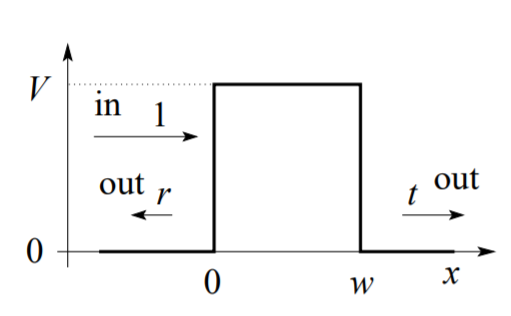
\includegraphics[scale=1]{3_7.PNG}
    \end{minipage}
    \begin{minipage}{0.5\textwidth}
        \captionsetup{font={Large}}
        \caption{The scattering matrix S transforms the incident amplitudes (here 1 from the left) into the outgoing amplitudes, here a transmitted t (to the right) and a reflected one (to the left).}
    \end{minipage}
\end{figure}
The amplitudes $r$ and $t$ are called reflection and transmission amplitudes. Consider a potential barrier between $x = 0 $and $x = w$ and a wave incident from the left with $a = 1$, e.g. Fig. 3.7; then a wave $t exp [ik (x - w)]$ is transmitted and a wave $r exp (-ikx)$ is reflected. (For a (parity) symmetric problem, with $\Psi(x)$ also $[P\Psi] (x ) = \Psi (-x)$ a solution, which describes a wave entering from the right and one recognizes immediately that $t+0 = t$ and $r_0 = r$ must be.) The phase $2φ$ of the reflection coefficient $r = | r |$ Within the quasi-classical approximation, $exp (i2φ)$ assumes the value $φ = \pi / 4$ for a linearly increasing potential; for an infinitely high potential, $φ = \pi / 2$, and the incident and reflected waves cancel out at the edges, $r = -1$ for the total reflection.\\
The form (3.22) can be diagonalized, 
%公式3.23
\begin{equation}
\begin{aligned} S_{D}=\left(\begin{array}{cc}{r+t} & {0} \\ {0} & {r-t}\end{array}\right)=\sqrt{\frac{t}{t^{*}}}\left(\begin{array}{cc}{e^{\pm i \varphi}} & {0} \\ {0} & {-e^{\mp i \varphi}}\end{array}\right) \\=\left(\begin{array}{cc}{e^{i(\delta \pm \varphi)}} & {0} \\ {0} & {-e^{i(\delta \mp \varphi)}}\end{array}\right) \end{aligned}
\end{equation}
with $t = |t|e^{i\delta},\delta$ is the phase of $t$ and $\varphi = arctan (| r | / | t |)$. (In a first step one finds the eigenvalues $​​r \pm t$. The unitarity relations $|t|^2+|r|^2=1, \text{ and } t^*r+r^*t=0$ imply that $| r \pm t |^2 = 1$. With the approach $t = | t | exp (i\delta), r = | r | exp (i\chi$ follows from $t^*r+r^*t = 0$, that $\chi = \delta \pm \pi / 2 + 2n\pi$. This yields eigenvalues ​​in the form $r + t = exp (i\delta) [(\pm i) | r | + | t |]$ and $r - t = exp (i\delta) [(\pm i) | r | - | t |]$. With $\varphi \equiv arctan (| r | / | t |)$ one finds the result $r + t = exp [i (\delta \pm \varphi)], r -t = - exp [i (\delta\mp\varphi)]$; the sign of $varphi$ results from the continuity of the solutions and changes with resonances ($r = 0$, note that then the phase $\chi = \delta \pm \pi / 2$ of $r$ also jumps by $\pi$), cf. the example of scattering at two $\delta$-potentials in Fig. 3.21)

\section{particles in the pot}
A potential well as shown in Fig. 3.8 binds states in a number determined by the potential depth V. The Heisenberg uncertainty principle gives us the energy scale of the problem: with Δx ≈ w Δp ~ ~ / w and we find the energy E0 = ~ 2 / 2mw2. The bound states in the potential well
%图 3.8
\begin{figure}[ht]
    \begin{minipage}{0.5\textwidth}
        \centering
        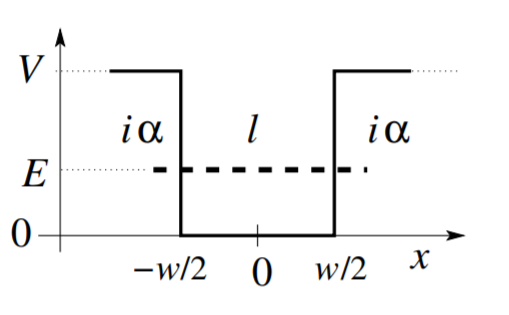
\includegraphics[scale=1]{3_8.PNG}
    \end{minipage}
    \begin{minipage}{0.5\textwidth}
        \captionsetup{font={Large}}
        \caption{Potential pot of width $w$ and depth $v$.}
    \end{minipage}
\end{figure}
can be found with the help of transfer matrix formalism. We construct the transfer matrix from the corresponding three elements,
%公式
$$
\begin{aligned}\left(\begin{array}{l}{a} \\ {b}\end{array}\right) &=\frac{1}{4}\left(\begin{array}{cc}{1+\frac{1}{i \kappa}} & {1-\frac{1}{i \kappa}} \\ {1-\frac{1}{i \kappa}} & {1+\frac{1}{i \kappa}}\end{array}\right)\left(\begin{array}{cc}{e^{-i l w}} & {0} \\ {0} & {e^{i l w}}\end{array}\right)\left(\begin{array}{cc}{1+i \kappa} & {1-i \kappa} \\ {1-i \kappa} & {1+i \kappa}\end{array}\right)\left(\begin{array}{c}{A} \\ {B}\end{array}\right) \\ &=M\left(\begin{array}{c}{A} \\ {B}\end{array}\right) \end{aligned}
$$
where $\kappa ≡ \alpha / l, \alpha = \sqrt{2m(V-E)}/\hbar, l=\sqrt{2mE}/\hbar$. With some trigonometry we find the transfer matrix
%公式 3.24
\begin{equation}
M=\left(\begin{array}{cc}{\cos l w-\sinh y \sin l w} & {-\cosh y \sin l w} \\ {\cosh y \sin l w} & {\cos l w+\sinh y \sin l w}\end{array}\right)
\end{equation}
with $y = - \operatorname{ln} \kappa$ and
%公式 3.25
\begin{equation}
    \sinh y=\frac{1}{2}\left(\frac{1}{\kappa}-\kappa\right), \quad \cosh y=\frac{1}{2}\left(\frac{1}{\kappa}+\kappa\right)
    \end{equation}
%Page85
We find the bound states by asking for normability. Accordingly, no exponentially growing components can occur, which is why the amplitudes a and B must disappear (no 'einfallende' particles),
%公式 3.26
\begin{equation}
\left(\begin{array}{l}{a} \\ {b}\end{array}\right)=\left(\begin{array}{l}{0} \\ {b}\end{array}\right),\left(\begin{array}{c}{A} \\ {B}\end{array}\right)=\left(\begin{array}{c}{A} \\ {0}\end{array}\right)
\end{equation}
This constraint forces the disappearance of the matrix element $M_{11}$ and we get the condition
%公式 3.27
\begin{equation}
    \cos l w=\sinh y \sin l w
    \end{equation}
which can be rewritten as$ cot x = [cot (x / 2) - tan (x / 2)] / 2$ and the relation (3.25)
%公式 3.28
\begin{equation}
    2 \cot l w=\cot (l w / 2)-\tan (l w / 2)=1 / \kappa-\kappa
    \end{equation}
With $cot x = 1 / tan x$ we ​​obtain the simpler transcendental equations
%公式 3.29
\begin{equation}
    \cot \frac{l w}{2}=-\kappa \quad \text { and } \quad \tan \frac{l w}{2}=\kappa
    \end{equation}
which can be solved graphically. For this we define new coordinates $\xi = lw / 2$ and $\eta = \alpha w / 2$ and find the relations
%公式 3.30
\begin{equation}
    \xi \cot \xi=-\eta, \quad \xi \tan \xi=\eta
    \end{equation}
The parameters $\xi = w\sqrt{2mE}/2\hbar$ and $\eta = w\sqrt{2m(V-E)}/2\hbar$ are linked via energy $E$ and potential $V$ and we get the second relation
%公式 3.31
\begin{equation}
    \xi^{2}+\eta^{2}=\frac{m w^{2} V}{2 \hbar^{2}} \overset{E_{0}=\hbar^{2} /2m w^{2}}{=} \frac{V}{4 E_{0}}
    \end{equation}
Figure 3.9 (a) illustrates the graphical solution to the problem. The solutions with even and odd numbers of nodes result alternately from the two transcendental equations; the energies result from the values ​​of $\xi$ via
%公式 3:32
\begin{equation}
    E=\frac{\hbar^{2} l^{2}}{2 m}=4 E_{0} \xi^{2}
\end{equation}
with the energy scale $E_0 = \hbar^2 / 2mw^2$; the associated eigenvalues ​​/ functions are shown in Figure 3.9 (b) and (c). An increase of $\xi$ by $\pi / 2$ gives another bound state if $\xi$ remains below the radius $\sqrt{V} / 4E_0$ of the circle (3.31). This immediately results in the maximum number of bound states nbound = $n_{bound}=\lfloor 2\xi/\pi\rfloor+1=\lfloor\sqrt{V/E_0}/\pi\rfloor+1$.
%page86
%图 3.9
\begin{figure}[ht]
        \centering
        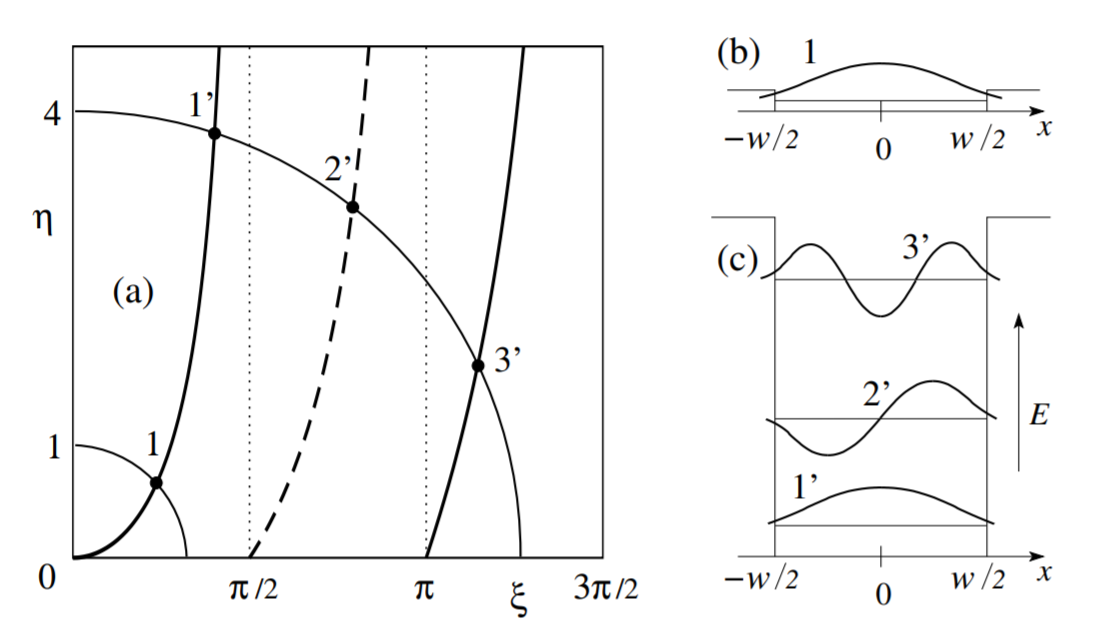
\includegraphics[scale=1]{3_9.PNG}
        \captionsetup{font={Large}}
        \caption{Energy eigenvalues and eigenfunctions for potential pots of depth $V = 4E_0$ and $V = 64E_0$. (a) Graphical solution of the transcendental equation with $\xi$ tan $\xi$ (straight solutions, solid lines) and $\xi$ cot $\xi$ (odd solutions, dashed lines). (b) Solution for the shallow pot with $V = 4E_0$, (c) Solutions for the deep pot with $V = 64E_0$.}
\end{figure}
\subsection{Parity}
For $V\to\infty$ results in wave functions of the form $\propto \operatorname{sin} (n\pi x / w)$ and $\propto \operatorname{cos} (n\pi x / w)$, cf. Section 1.6.2; these are odd and even in $x$. This symmetry for the wave functions also holds for potential heads of finite depth, that is, $V <\infty$; it is a consequence of the symmetry $x\longleftrightarrow -x$ of the Hamiltonian. We define the (symmetry) operator $P$, the parity operator
%公式 3:33
\begin{equation}
    (P \Psi)(x)=\Psi(-x), \quad\langle x|P| \Psi\rangle=\langle- x | \Psi\rangle
    \end{equation}
The Hamiltonian $H$ commutes with $P$, that is, $H$ is invariant under the exchange $x \longleftrightarrow -x$ since we chose $V (x)$ symmetrically, $V (x) = V (-x)$. In particular, the kinetic term is invariant under $x \longleftrightarrow -x: \partial_x^2\to (-\partial_x)^2=\partial_x^2$, and it is explicit that $\langle | HP | \Psi\rangle = \langle x | P H | \Psi\rangle$ for all $\Psi$ and all $x$,

%Page 87
%公式 3:34
\begin{equation}
\begin{aligned}\langle x|H P| \Psi\rangle &=\left[-\left(\hbar^{2} / 2 m\right) \partial_{x}^{2}+V(x)\right]\langle x|P| \Psi\rangle \\ &=\left[-\left(\hbar^{2} / 2 m\right) \partial_{x}^{2}+V(x)\right]\langle- x | \Psi\rangle \\ &=\left[-\left(\hbar^{2} / 2 m\right) \partial_{x}^{2}+V(-x)\right]\langle- x | \Psi\rangle \\
&=\langle- x|H| \Psi\rangle=\langle x|P H| \Psi\rangle
\end{aligned}
\end{equation}
$P$ is an involution, $P_2 = \mathbb{I}$, resulting in eigenvalues $\pm 1$. Since $H$ and $P$ commute, cf. the discussion on page 64, we can simultaneously diagonalize $H$ and $P$, that is, we can choose eigenvectors to $H$, which are at the same time eigenvectors to $P$ and thus either even or odd in $x$. Since $H$ has no other symmetry, dimEigEn = $1$ and our eigenfunctions to $H$ are automatically even or odd: the solutions to $\xi tan \xi= \eta$ are even (it obviously always exists at least one such solution) while the solutions to $\xi cot\xi = -\eta$ are odd. For $V <\pi^2E_0$ there is only one bound state. In special cases (or, more generally, if there is an additional symmetry), Dim $Eig_{E_n}> 1$, for example, could be a symmetric double-well potential with an infinitely high partition. Let the potential $V (x) = V (-x)$ be symmetric, then with $\phi n (x)$ we also get $\phi n (-x)$ as a solution. If dim $Eig_{E_n} = 1$ then $\phi n (-x) = (+ \text{ or } -) \phi n (x)$ and we find (anti-) symmetrical eigenfunctions. If dim$Eig_{E_n} ≥ 2$ then the linear combinations $\varphi_{g, u} = [\varphi_n (x) \pm \varphi_n (-x)] / \sqrt{2}$ define even or odd eigenfunctions in $Eig_{E_n}$.
In summary, let $H$ be symmetric with interchange $x \longleftrightarrow -x, [H, P] = 0, P$ is the parity operator, $P^2 = \mathbb{I}$. Let $\Psi$ be a solution to $H\Psi = E\Psi$, then also $\Phi\equiv P\Psi$ solution of the eigenvalue problem with the same energy, $H\Phi = HP\Psi = P H\Psi = P E\Psi = E\Phi$. It is either $\langle\Psi,\Phi\rangle = 0, \Phi ⊥ \Psi$, and $\Psi, \Phi $span at least one two-dimensional eigenspace ($\to$ (anti -) - symmetrize the wavefunctions) or $\Phi = \alpha\Psi=P\Psi\to P\Psi=\pm\Psi$ and $\Psi$ either even or odd. You can always find states that diagonalize both $H$ and $P$.
\section{Tunnel effect}
The tunnel effect describes the 'propagation' of a particle through an energetically forbidden zone, cf. Fig. 3.10, a pure quantum effect that is classically forbidden. Again, the tunneling effect can be described with the transfer matrix formalism; with $\kappa = k / \alpha$ we compose the transfer matrix $M$ from three elements and find it
%图 3.10
\begin{figure}[ht]
    \begin{minipage}{0.5\textwidth}
        \centering
        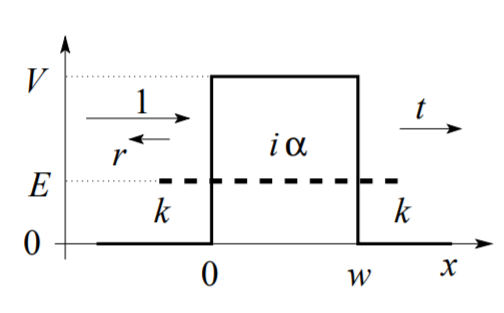
\includegraphics[scale=1]{3_10.PNG}
    \end{minipage}
    \begin{minipage}{0.5\textwidth}
        \captionsetup{font={Large}}
        \caption{Tunnel effect: Particles can penetrate a potential barrier. $t$ and $r$ are transmission and reflection coefficients and we define $\kappa = k / \alpha$.}
    \end{minipage}
\end{figure}
%公式 3:35
\begin{equation}
    \begin{split}
    \left(\begin{array}{l}{a} \\ {b}\end{array}\right)&=\frac{1}{4}\left(\begin{array}{cc}{1-\frac{1}{i \kappa}} & {1+\frac{1}{i \kappa}} \\ {1+\frac{1}{i \kappa}} & {1-\frac{1}{i \kappa}}\end{array}\right)\left(\begin{array}{cc}{e^{\alpha w}} & {0} \\ {0} & {e^{-\alpha w}}\end{array}\right)\left(\begin{array}{cc}{1-i \kappa} & {1+i \kappa} \\ {1+i \kappa} & {1-i \kappa}\end{array}\right)\left(\begin{array}{c}{A} \\ {B}\end{array}\right)\\
    &=M\left(\begin{array}{c}
        {A}\\{B}
    \end{array}\right)\\
    \end{split}
\end{equation}
%公式 3:36
\begin{equation}
M=\left(\begin{array}{cc}{\cosh \alpha w+i \sinh y \sinh \alpha w} & {i \cosh y \sinh \alpha w} \\ {-i \cosh y \sinh \alpha w} & {\cosh \alpha w-i \sinh y \sinh \alpha w}\end{array}\right)
\end{equation}
with $y = - \operatorname{ln} \kappa$ and
%公式 3:37
\begin{equation}
\sinh y=\frac{1}{2}\left(\frac{1}{\kappa}-\kappa\right), \quad \cosh y=\frac{1}{2}\left(\frac{1}{\kappa}+\kappa\right)
\end{equation}
The transfer matrices (3.36) and (3.24) are $\alpha$ equivalent under the interchange $l\longleftrightarrow i\alpha$. The tunnel configuration can also be understood as a scattering configuration, with incident and reflected (backscatter) amplitude $a = l$ and $b = r$, as well as a transmitted (previously scattered) amplitude $t$.
%公式 3:38
\begin{equation}
\left(\begin{array}{l}{a} \\ {b}\end{array}\right)=\left(\begin{array}{l}{1} \\ {r}\end{array}\right), \quad\left(\begin{array}{l}{A} \\ {B}\end{array}\right)=\left(\begin{array}{l}{t} \\ {0}\end{array}\right)
\end{equation}
The combination with (3.36) leads us to the transfer matrix in the form
%公式 3:39
\begin{equation}
M=\left(\begin{array}{cc}{\frac{1}{t}} & {\frac{r^{*}}{t^{*}}} \\ {\frac{r}{t}} & {\frac{1}{t^{*}}}\end{array}\right)
\end{equation}
with the properties (by comparison with (3.36))
%公式 3:40
\begin{equation}
\begin{aligned} \frac{r^{*}}{t^{*}} &=-\frac{r}{t}, \quad|r|^{2}+|t|^{2}=1 \\ \operatorname{det} M &=\frac{1}{|t|^{2}}-\frac{|r|^{2}}{|t|^{2}}=1 \\ M^{-1} &=\left(\begin{array}{cc}{\frac{1}{t^{*}}} & {-\frac{r^{*}}{t^{*}}} \\ {-\frac{r}{t}} & {\frac{1}{t}}\end{array}\right)=\left(\begin{array}{cc}{\frac{1}{t^{*}}} & {\frac{r}{t}} \\ {\frac{r^{*}}{t^{*}}} & {\frac{1}{t}}\end{array}\right)=M^{*} \end{aligned}
\end{equation}
For the calculation of $M^{-1}$ we have the usual relation
%公式 3:41
\begin{equation}
A=\left(\begin{array}{ll}{a} & {b} \\ {c} & {d}\end{array}\right) \quad \Leftrightarrow \quad A^{-1}=\frac{1}{\operatorname{det} A}\left(\begin{array}{cc}{d} & {-b} \\ {-c} & {a}\end{array}\right)
\end{equation}
used. The transmission $(t)$ and reflection $(r)$ coefficients defined here are identical to those in the scattering matrix,
%公式 3:42
\begin{equation}
S=\left(\begin{array}{ll}{r} & {t} \\ {t} & {r}\end{array}\right)
\end{equation}
whereas the scattering matrix S connects the amplitudes $(a\quad B)$ and $(b\quad A)$, the transfer matrix $M$ transposes the amplitudes $(A\quad B)$ into $(a \quad b)$. Although all particles are classically reflected (note that $E <V$) can quantum mechanically penetrate particles through the forbidden region and propagate further for $x> w$: this is the tunneling effect. The probability for the tunneling process is given by
%公式 3:43
\begin{equation}
    |t|^{2}=\frac{1}{1+\cosh ^{2} y \sinh ^{2} \alpha w}\overset{{\left(\frac{1}{\kappa}+\kappa\right)^{2}}=\frac{V^{2}}{2}}{=} \frac{1}{1+\frac{V^{2} \sinh ^{2} \alpha w}{4 E(V-E)}}
    \end{equation}
We used the relations $cosh^2 \alpha w - sinh^2 \alpha w = 1$ and $cosh^2 \alpha w + sinh^2 y sinh^2 \alpha w = 1 + cosh^2 y sinh^2 \alpha w$. The tunnel amplitude is given too
%公式 3:44
\begin{equation}
    t=\frac{2 i k \alpha}{2 i k \alpha \cosh \alpha w-\left(\alpha^{2}-k^{2}\right) \sinh \alpha w}
    \end{equation}
With $\alpha w = w\sqrt{2m (V - E)} / \hbar = \sqrt{ (V - E)} / E_0$ and $E_0, E\ll V$ we obtain
%公式 3:45
\begin{equation}
    |t|^{2} \approx \frac{16 E}{V} e^{-2 \sqrt{V / E_{0}}}, \quad t \approx-4 i \sqrt{\frac{E}{V}} e^{-\sqrt{V / E_{0}}}
    \end{equation}
or
%公式 3:46
\begin{equation}
    |t|^{2} \approx \frac{16 E}{V} e^{-2 w \sqrt{2 m V} / \hbar}, \quad t \approx-4 i \sqrt{\frac{E}{V}} e^{-w \sqrt{2 m V} / \hbar}
    \end{equation}
The tunneling probability is exponentially small in the distance w and in the forbidden momentum $\propto \sqrt{V}: \sqrt{(V - E) / E_0} = \alpha w = (\text{ forbidden pulse }/\hbar) · \text{ path } = ΔpΔx / \hbar$. Thus, the Heisenberg uncertainty principle (HUP) is ultimately responsible for the tunneling process: A particle can 'survive' a distance $Δx ~ \hbar / Δp$ in the forbidden regime. The exponent $\alpha w = \int p dx / \hbar$ measures how strongly prohibited the process is.\\\\
It is interesting to plot the trajectories of the reflection and transmission amplitudes $r$ and $t$ in the complex plane as a function of the energy E of the incident particle, see Fig. 3.11 and these with the results in Fig. 3.21 for the double barrier in section 3.7. 2 compare.
%图 3.11
\begin{figure}[ht]
    \centering
    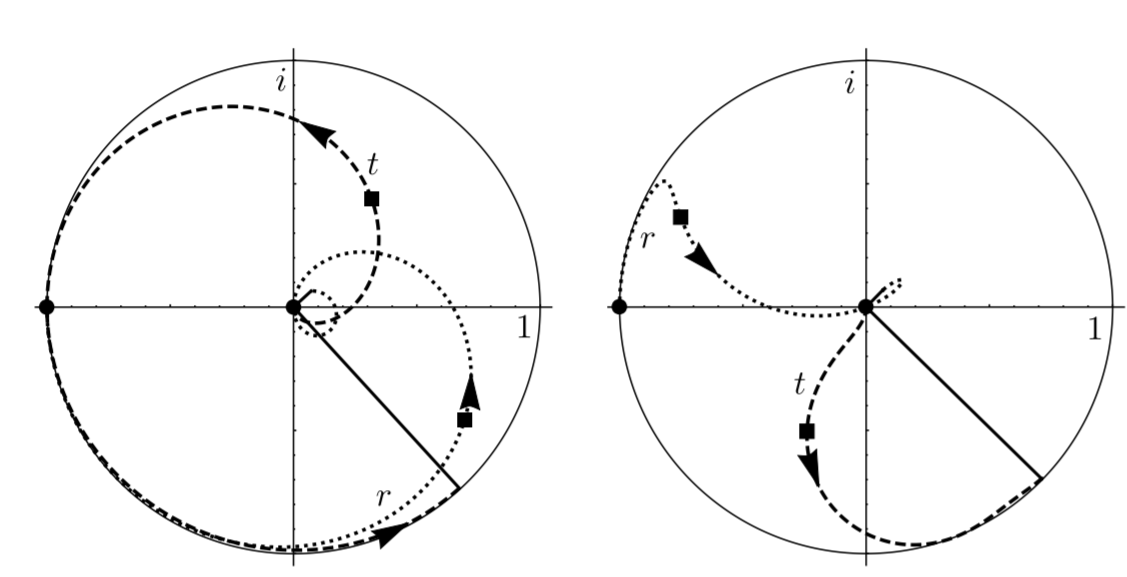
\includegraphics[scale=1]{3_11.PNG}
    \captionsetup{font={Large}}
    \caption{Trajectories of the reflection and transmission amplitudes $r$ (dotted) and $t$ (dashed) in the complex plane as a function of the energy $E$ of the incident particle ($E$ = curve parameter). The starting points at$ E = 0 (r = -1, t = 0)$ are marked by bold points $\bullet$. The marker $\blacksquare$ denotes the energy $E = V$ where the particle first hits the barrier can fly over. The vectors for $r$ and $t$ are orthogonal (according to $r^*t+t^*r=0$ for a symmetric potential). Left: $r$ and $t$ as defined in (3.38); the reflection coefficient $r$ follows the unit circle and falls through the center when $t = -1$ (first resonance); the transmission $t$ swings up to the unit circle and touches this in the resonances with energies $E> V$. Right: renormalized coefficients $r \to exp (-ikw) r$ and $t \to exp (-ikw) t$ reduced by the trivial propagation phase $kw$. The transmission $t$ approaches the asymptotic value 1
    by oscillating closer and closer to the unit circle.}
\end{figure}
The tunnel effect has multiple technical applications. On the one hand, these are 'everyday' effects such as the penetration of electrons (current) through oxide layers in semiconductors (electronics, transistors, see the work of Tsui \& Esaki, Appl. Phys. Lett., 22, 562 (1973), Sollner et al., Appl. Phys., Lett., 43, 588 (1983), Ricco \& Azbel, Phys., Rev. B, 29, 1970 (1984))., On the other hand, the effect has interesting applications such as the tunneling microscope (Binnig and Rohrer, Phys., Rev. Lett., 50, 120 (1983)), outlined in Figure 3.12.

%Page 91
%图 3.12
\begin{figure}[ht]
    \centering
    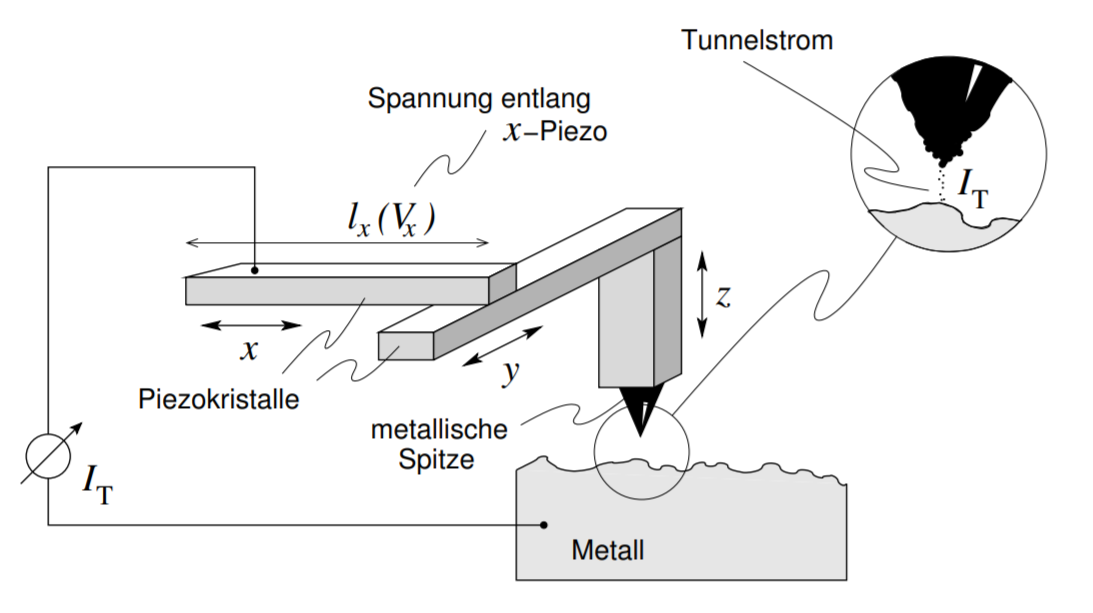
\includegraphics[scale=1]{3_12.PNG}
    \captionsetup{font={Large}}
    \caption{Tunneling microscope (Binnig \& Rohrer, IBM): The tunneling current IT flows from the metal tip of the microscope to the surface under investigation. The current $I_T$ depends sensitively (exponentially) on the distance tip-to-surface and can thus be used as control parameters: The current $I_T$ is transformed into a voltage $V_z (x, y)$ which manipulates the piezocrystal along $z$, so $I_T$ stays constant. The crystals along the $x, y$ plane serve to shift the tip ('scanning'). The potential relief $V_z (x, y)$ then serves as the elevation map of the surface.}
\end{figure}
\section{$\delta$-potential}
The solution for the $\delta$-potential, see Fig. 3.13, involves a special transfer matrix which is also useful in other situations, e.g. for the solution of the Kronig-Penney model or for the problem of the double barrier. To solve is the eigenvalue problem with the Hamiltonian
%公式 3:47
\begin{equation}
    H=-\frac{\hbar^{2}}{2 m} \partial_{x}^{2}+V_{0} \delta(x)
    \end{equation}
where the $\delta$-function forces special boundary conditions at 0. Note the units of [$V$] = energy, whereas that of [$V_0$] = energy · length. To get the boundary conditions at $\Psi_0 (x)$ at $x = 0$
integrate $H\Psi$ over the interval $[-\epsilon, \epsilon], \epsilon\to 0$, around 0,

%Page 92
%图 3.13
\begin{figure}[ht]
    \begin{minipage}{0.5\textwidth}
        \centering
        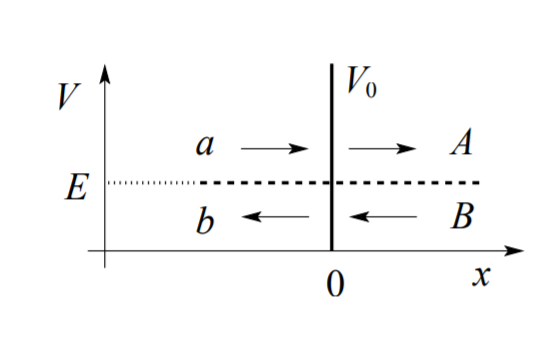
\includegraphics[scale=1]{3_13.PNG}
    \end{minipage}
    \begin{minipage}{0.5\textwidth}
        \captionsetup{font={Large}}
        \caption{Delta potential of the strength
        $V_0$.}
    \end{minipage}
\end{figure}
%公式 3:48
\begin{equation}
\begin{aligned} \int_{-\varepsilon}^{\varepsilon}\left[-\frac{\hbar^{2}}{2 m} \Psi^{\prime \prime}+V_{0} \delta(x) \Psi\right] d x &=\frac{\hbar^{2}}{2 m}\left(\Psi_{l}^{\prime}-\Psi_{r}^{\prime}\right)+V_{0} \Psi(0) \\ &=\int_{-\varepsilon}^{\varepsilon} E \Psi(x) d x=0 \end{aligned}
\end{equation}
With $\Psi_l (0) = \Psi_r(0)$ regular in 0 and (3.48) we get the equation system
%公式 3:49
\begin{equation}
\begin{aligned} a+b &=& A+B, & \quad k=\sqrt{2 m E} / \hbar \\ a(1-2 i v / k)-b(1+2 i v / k) &=&A-B, &\quad v=m V_{0} / \hbar^{2} \end{aligned}
\end{equation}
in matrix notation
%公式 3:50
\begin{equation}
\left(\begin{array}{l}{a} \\ {b}\end{array}\right)=\left(\begin{array}{cc}{1+i v / k} & {i v / k} \\ {-i v / k} & {1-i v / k}\end{array}\right)\left(\begin{array}{c}{A} \\ {B}\end{array}\right)
\end{equation}
the same result is obtained from (3.36) with $V · w = V0 = \text{ const. and }w \to 0,$
%公式 3:51
\begin{equation}
\begin{aligned} \alpha w &=\sqrt{2 m\left(w V_{0}-E w^{2}\right)} / \hbar \rightarrow 0 \\ \kappa &=\alpha / k=\sqrt{2 m\left(V_{0} / w-E\right)} / \hbar k \rightarrow \infty \end{aligned}
\end{equation}
In the following we consider both attractive and repulsive potentials:
\subsection{$V_0 <0$, bound state}
For bound states, the boundary condition applies
%公式 3:52
\begin{equation}
\left(\begin{array}{l}{a} \\ {b}\end{array}\right)=\left(\begin{array}{l}{0} \\ {b}\end{array}\right) \quad \text { and } \quad\left(\begin{array}{l}{A} \\ {B}\end{array}\right)=\left(\begin{array}{l}{A} \\ {0}\end{array}\right)
\end{equation}
%page 93
it produces the condition $1 + iv / k = 0$ which requires that $k \to i\alpha = i\sqrt{2m | E |} / \hbar$ be purely imaginary, which corresponds to a negative energy $E <0$. The energy eigenvalue results from
%公式 3:53
\begin{equation}
    1=-\frac{i v}{k}=\frac{m\left|V_{0}\right| \hbar}{\hbar^{2} \sqrt{2 m|E|}} \rightarrow E=-\frac{m V_{0}^{2}}{2 \hbar^{2}}
    \end{equation}
and we find for every $V_0 <0$ exactly one bound state (note that $dim = 1$), see Fig. 3.14.
%图 3.14
\begin{figure}[ht]
    \begin{minipage}{0.5\textwidth}
        \centering
        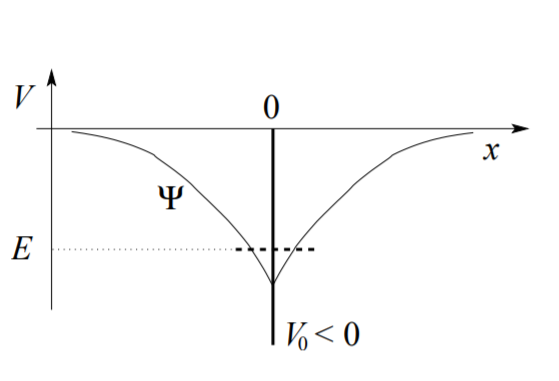
\includegraphics[scale=1]{3_14.PNG}
    \end{minipage}
    \begin{minipage}{0.5\textwidth}
        \captionsetup{font={Large}}
        \caption{The attractive $\delta$-potential in 1D binds exactly a condition. The kink in the wave function at $x = 0$ produces the compensating $\delta$-function after two derivatives. Compare also with the kink in the 1D Green's function to the operator $\mathcal{L}=\partial_x^2$}
    \end{minipage}
\end{figure}
\subsection{$V_0> 0$, scattering condition}
The transmission amplitude is
%公式 3:54
\begin{equation}
    t=\frac{1}{1+i v / k}, \quad|t|^{2}=\frac{1}{1+m V_{0}^{2} / 2 \hbar^{2} E}\overset{V_0 \text{ gross }}{\approx}\frac{2\hbar^2 E}{mV_0^2}
    \end{equation}
This result also follows from (3.43) with sinh αw ≈ αw and the substitutionV $-E \to V_0 / w-E \approx V_0 / w$. The relevant energy scale in the problem is given by $E = mV_0^2/2\hbar^2\sim V^2 / 4E_0$.
\section{Resonances}
We consider a pot potential as sketched in Fig. 3.15. The energy of the particle is positive this time, corresponding to a scattering configuration. Classically, we expect the particle to fly over the potential well - the quantum mechanical result is different.
Propagation again involves three subelements
%公式 3:55
\begin{equation}
\left(\begin{array}{l}{a} \\ {b}\end{array}\right)=\frac{1}{4}\left(\begin{array}{cc}{1+\frac{1}{\kappa}} & {1-\frac{1}{\kappa}} \\ {1-\frac{1}{\kappa}} & {1+\frac{1}{\kappa}}\end{array}\right)\left(\begin{array}{cc}{e^{-i l w}} & {0} \\ {0} & {e^{i l w}}\end{array}\right)\left(\begin{array}{cc}{1+\kappa} & {1-\kappa} \\ {1-\kappa} & {1+\kappa}\end{array}\right)\left(\begin{array}{l}{A} \\ {B}\end{array}\right)
\end{equation}
%Page94
%图 3.15
\begin{figure}[ht]
    \begin{minipage}{0.5\textwidth}
        \centering
        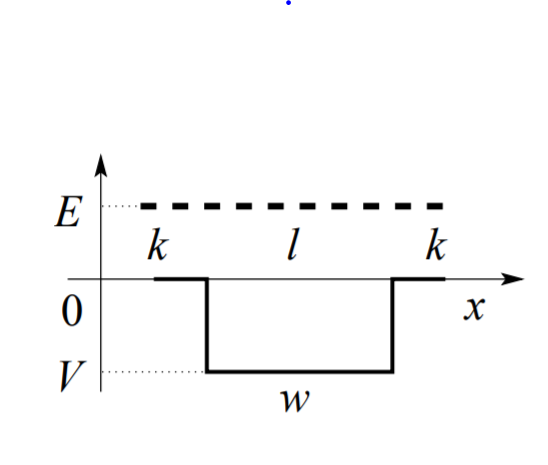
\includegraphics[scale=1]{3_15.PNG}
    \end{minipage}
    \begin{minipage}{0.5\textwidth}
        \captionsetup{font={Large}}
        \caption{Pot potential of depth V and width w which generates stray resonances. We define
        $k=\sqrt{2mE}/\hbar,l=\sqrt{2m(E-V)}/\hbar,\text{ and }\kappa=k/l.$}
    \end{minipage}
\end{figure}
and we find the transfer matrix for the scattering problem in the mold
%公式 3:56
\begin{equation}
M=\left(\begin{array}{cc}{\cos w l-i \cosh y \sin w l} & {-i \sinh y \sin w l} \\ {i \sinh y \sin w l} & {\cos w l+i \cosh y \sin w l}\end{array}\right)
\end{equation}
with $y = - ln \kappa$ and
%公式 3:57
\begin{equation}
    \sinh y=\frac{1}{2}\left(\frac{1}{\kappa}-\kappa\right), \quad \cosh y=\frac{1}{2}\left(\frac{1}{\kappa}+\kappa\right)
    \end{equation}
Printed by reflection and transmission amplitudes we can write
%公式 3:58
\begin{equation}
\left(\begin{array}{l}{a} \\ {b}\end{array}\right)=\left(\begin{array}{l}{1} \\ {r}\end{array}\right)=M\left(\begin{array}{l}{t} \\ {0}\end{array}\right)=M\left(\begin{array}{l}{A} \\ {B}\end{array}\right)
\end{equation}
with
%公式 3:59
\begin{equation}
\begin{aligned} M &=\left(\begin{array}{cc}{\frac{1}{t}} & {\frac{r^{*}}{t^{*}}} \\ {\frac{r}{t}} & {\frac{1}{t^{*}}}\end{array}\right) \\ t &=\frac{1}{\cos w l-i \cosh y \sin w l} \end{aligned}
\end{equation}
The transmission probability is
%公式 3.60
\begin{equation}
    |t|^{2}=\frac{1}{1+\left[\sin ^{2}(w l) V^{2}\right] / 4 E(E-V)}
    \end{equation}
and $| t |^2 <1$ in general. This means that quantum-mechanical particles can also be reflected at potential with energies $E> V (x)$, which would not be classically possible; Quantum mechanical and classical scattering processes are different. Perfect transmission occurs under the condition $| t |^2 = 1$; this is the case for $sin^ 2 wl = 0$. The condition $l = n\pi / w$,
then gives the associated energies
%公式 3.61
\begin{equation}
    E_{\mathrm{res}}=\frac{\hbar^{2} \pi^{2}}{2 m w^{2}} n^{2}+V=E_{0}(n \pi)^{2}+V
    \end{equation}
The number of bound states follows from the condition $E_0 (n\pi)^2 + V <0, n> \sqrt{| V | / E0 /} \pi$, and we find the minimum $n$ for a resonance,
%公式 3.62
\begin{equation}
    n_{\min }>\lceil\sqrt{|V| / E_{0}}\rceil= n_{\text {bound }}
    \end{equation}
A pretty application example is the resonant tunnel diode, cf. Fig. 3.16. The transmission amplitude has the form
%图 3.16
\begin{figure}[ht]
    \begin{minipage}{0.5\textwidth}
        \centering
        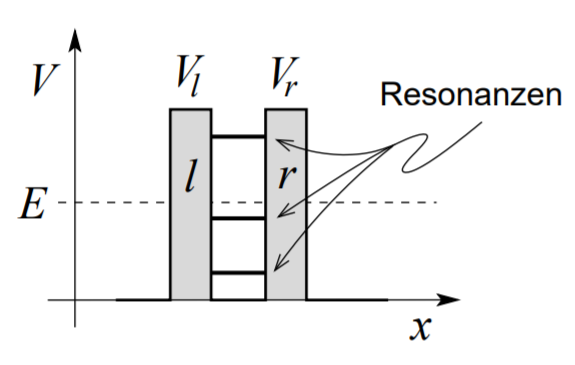
\includegraphics[scale=1]{3_16.PNG}
    \end{minipage}
    \begin{minipage}{0.5\textwidth}
        \captionsetup{font={Large}}
        \caption{Double barrier for the resonant tunnel diode.}
    \end{minipage}
\end{figure}
%公式 3.63
\begin{equation}
    t(E)=\frac{C_{0}}{C_{1} T_{l} T_{r}+C_{2} T_{l} / T_{r}+C_{3} T_{r} / T_{l}+C_{4} / T_{l} T_{r}}
    \end{equation}
with the transmission coefficients $T_l$ and $T_r$ for the left and right barrier. We choose $V_l$, $V_r$ large, $E$ small, so that $T_l, T_r \ll 1$. Thus, $(E) ≈ (C_0 / C_4) T_lT_r \ll 1$, unless $C_4 = 0$. If one chooses $E$ such that $C_4 (E) = 0$ vanishes, then $t (E) \approx CT_{min} / T_{max} \sim 1$ for $T_l = T_r$ (symmetric barriers). The resonant tunnel diode RTD is a useful device with negative differential resistance (NDR) in certain voltage ranges, cf. Fig. 3.17.
3.7 Analyticity
The analytic structure of the transmission coefficient $t (p)$ or $t (E)$ as a function of the momentum p or the energy E provides information about bound states and resonances. For this we set the functions $t (p)$ and $t (E)$ into the complex $p$ and $e$ plane. The relationship between the momentum $p = \sqrt{2mE}$ and the energy $E$ is given by
%公式 3.64
\begin{equation}
    E=\frac{p^{2}}{2 m}, \quad p=\sqrt{2 m E}
    \end{equation}
with the complex root defined via
%公式 3.65
\begin{equation}
    \sqrt{z}=\sqrt{|z|} e^{i \arg (z) / 2} \operatorname{mit} \arg z \in[0,2 \pi)
    \end{equation}
%图 3.17
\begin{figure}[ht]
        \centering
        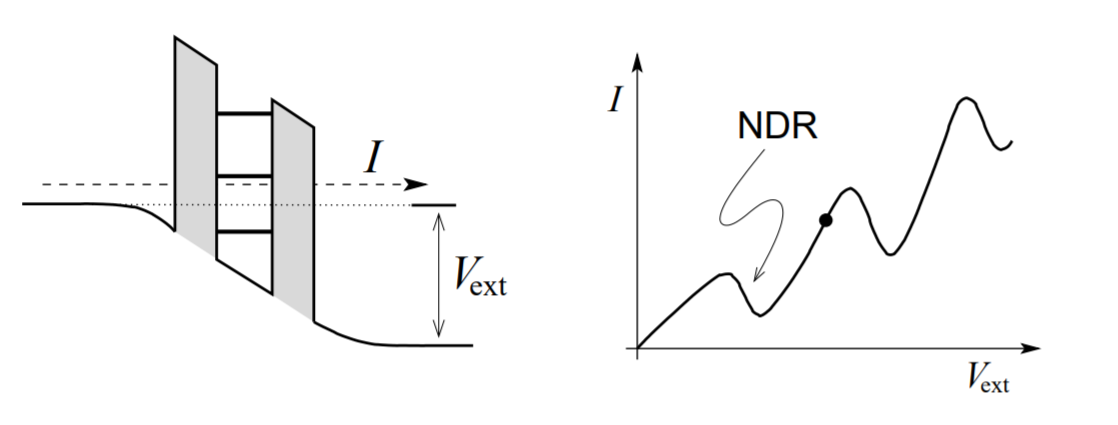
\includegraphics[scale=1]{3_17.PNG}
        \captionsetup{font={Large}}
        \caption{Left: Double barrier of the resonant tunnel diode under voltage Vext. The transmission through the double barrier increases dramatically when electrons in the left conductor are resonant to a quasi-bound state within the double barrier. Right: I-V characteristic of a resonant tunnel barrier with resonance peaks. The negative differential resistance (NDR) is used technologically.}
\end{figure}
and is shown in Fig. 3.18. The physical plane is the first Riemann plane of $E$ with $\operatorname{Im} p> 0$.
%图 3.18
\begin{figure}[ht]
    \centering
    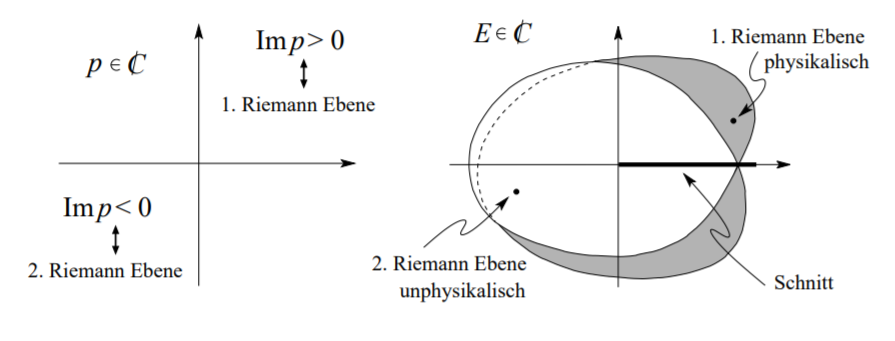
\includegraphics[scale=1]{3_18.PNG}
    \captionsetup{font={Large}}
    \caption{Complex $p$ plane and its mapping into the complex $E$ plane with two Riemann surfaces.}
\end{figure}
\subsection{Poles of $t$, Zeros $t^{-1} = 0$}
 Examination of the zeros of $t^{-1}$ or poles of $t$ for the pot potential gives the conditions
%公式 3.66
\begin{equation}
    2 i k l t^{-1}=2 i k l \cos l w+\left(k^{2}+l^{2}\right) \sin l w=0
    \end{equation}
Equation (3.66) is satisfied when
%公式 3.67
\begin{equation}
    2 \cot l w=\cot \frac{l w}{2}-\tan \frac{l w}{2}=\frac{i k}{l}-\frac{l}{i k}\\
    \cot \frac{l w}{2}=\frac{i k}{l} \text {  or  } \tan \frac{l w}{2}=-\frac{i k}{l}
    \end{equation}
The comparison with (3.29) shows that these conditions give just the bound states, where $ik$ just equals $-\alpha$ for a negative energy $E <0$,
%公式 3.68
\begin{equation}
\begin{aligned} i k &=\frac{i}{\hbar} \sqrt{2 m E} \stackrel{E<0}{=}-\alpha, \quad \alpha=\sqrt{2 m|E|} / \hbar \\ \Rightarrow \cot \frac{l w}{2} &=\frac{-\alpha}{l}, \quad \tan \frac{l w}{2}=\frac{\alpha}{l} \end{aligned}
    \end{equation}
Thus the poles of $t$ lie on the imaginary axis in $p$, $p \in i\mathbb{R}^+$ or on the negative semiaxis $E <0$. The poles of t lie in the first Riemann plane; they are physically relevant and describe bound states. 
\subsection{Resonances in $t, t \approx 1$}
 Next we investigate t (E) near a resonance, $wl ≈ n\pi$ and $E_n = \hbar^2\pi^2 n^2 / 2mw^2$,
%公式 3.69
\begin{equation}
    \frac{1}{t}=\cos w l\left[1-\frac{i}{2}\left(\frac{k}{l}+\frac{l}{k}\right) \tan w l\right] \approx \pm 1
    \end{equation}
It is $\operatorname{cos} wl \approx 1$ and we can develop the second factor in $E - E_n$ (use that tan $wl | E_n = 0$)
%公式 3.70
\begin{equation}
    1-\frac{i}{2} \frac{d}{d E}\left[\left(\frac{k}{l}+\frac{l}{k}\right) \tan w l\right]_{E_{n}}\left(E-E_{n}\right) \equiv 1-\frac{2 i}{\Gamma}\left(E-E_{n}\right)
    \end{equation}
%公式 3.71
\begin{equation}
    \operatorname{with} \quad \frac{4}{\Gamma}=\left.\left(\frac{k}{l}+\frac{l}{k}\right) \frac{d w l}{d E}\right|_{E_{n}}
    \end{equation}
Thus we obtain for $t(E)$ a rational function generated by a pole at $E = E_n - i\Gamma / 2$ in the lower complex half-plane,
%公式
$$
    t(E) \cong \frac{\pm i \Gamma / 2}{E-\left(E_{n}-i \Gamma / 2\right)}
$$
We obtain the pole at $E = E_n - i\Gamma / 2$ by analytically continuing $t (E)$ through the cut in $\mathbb{R}^+$ into the lower half-plane, so that this pole comes to rest in the second Riemann plane and is therefore unphysical.\\
This means that this pole does not correspond to a bound state. What we see on $E\in \mathbb{R}^+$ from this pole is a quasi-bound state, a resonance. The distance $\Gamma / 2$ from the axis $\mathbb{R}^+$ gives us the lifetime of the resonance / the quasi-bound state,
%公式 3.72
\begin{equation}
\begin{aligned} \Psi(x, t) \propto e^{-i E t / \hbar} &=e^{-i\left(E_{n}-i \Gamma / 2\right) t / \hbar} \\ &=e^{-i E_{n} t / \hbar} e^{-\Gamma t / 2 \hbar} \end{aligned}
\end{equation}
All of these properties (poles, resonances and phase shifts) are generally valid structures of the scattering matrix, which reappear in the scattering theory in dim = 3. Figure 3.19 summarizes these results.
We can write the amplitude $t (E)$ as a product of modulus and phase,
%公式 3.73
\begin{equation}
    t(E)=|t| e^{i \delta(E)}
    \end{equation}
the magnitude square $| t (E) |^2$ is described by a Lorentz curve, cf. Fig. 3.20 (a),
%公式 3.74
\begin{equation}
    |t|^{2} \cong \frac{\Gamma^{2} / 4}{\left(E-E_{n}\right)^{2}+\Gamma^{2} / 4}
    \end{equation}
and for the phase we get (modulo $\pi$)
%公式 3.75
\begin{equation}
    \delta(E)=\arctan \left[2\left(E-E_{n}\right) / \Gamma\right]
    \end{equation}
At each resonance, the phase $\delta (E)$ increases by $\pi$, cf. Fig. 3.20 (b). The value $\delta (E = 0)$ is related to the number of bound states, cf. Levinson's Theorem [e.g. in M. Sassoli de Bianchi, J. Math. Phys. 35, 2719 (1994)], $\delta (0) = (nbound - 1/2) \pi$ (case without $E = 0$ solution).
%图 3.19
\begin{figure}[ht]
    \centering
    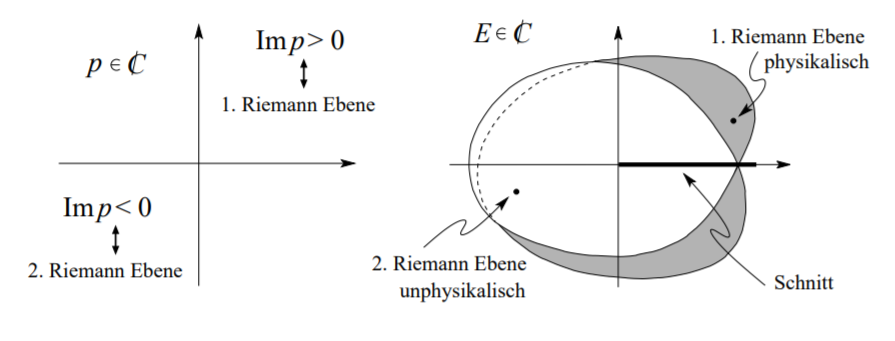
\includegraphics[scale=1]{3_18.PNG}
    \captionsetup{font={Large}}
    \caption{Bound states produce a pole in $t (p), t (E)$ for $p \in i\mathbb{R}^+, E <0$ in the 1st Riemann plane. Resonances appear as poles in the transmission amplitude $t (E)$ for energies $E$ in the lower complex half-plane of the 2nd Riemann plane; they are unphysical.}
\end{figure}
%图 3.20
\begin{figure}[ht]
    \begin{minipage}{0.5\textwidth}
        \centering
        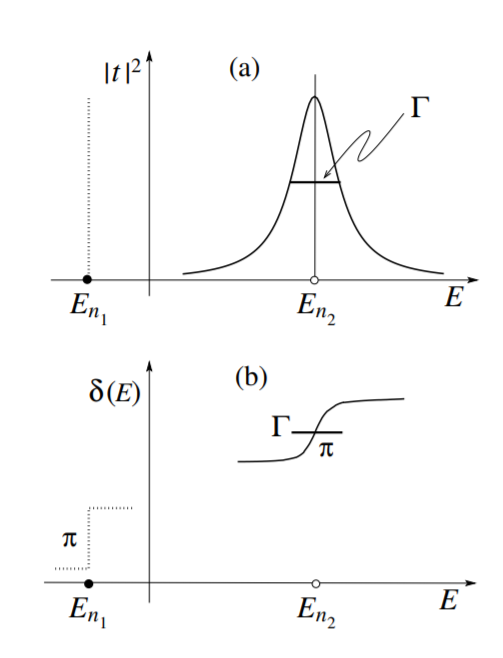
\includegraphics[scale=1]{3_20.PNG}
    \end{minipage}
    \begin{minipage}{0.5\textwidth}
        \captionsetup{font={Large}}
        \caption{(a) transmission probability $\mid t(t)\mid^2$ at a resonance $E_{n_2}> 0$; a bound state at $E_{n_1} <0$ corresponds to a $\delta$-function. (b) phase shift $\delta(E)$ in $t (E)$ via a resonance; the jump in $\pi$ is lubricated over the width $Gamma$ (= inverse lifetime of the resonance). A bound state corresponds to a sharp level.}
    \end{minipage}
\end{figure}
In Figure 3.21, the transmission amplitudes are $t = | t | exp (i\bar{\delta})$ and the associated reflection amplitude $r = | r | exp (i\bar{\chi})$ for the case of two repulsiver $\delta$ functions at a distance $w$. The phases $\bar{\delta} = \delta - kw \text{ and } \bar{\chi}=\chi-kw$ of the transmission and reflection amplitudes $t$ and $r$ involve the additional shift $-kw$; one finds this correction by using a single reference point instead of different reference points for the plane waves $\Psi_l$ and and $\Psi_r$, cf. (3.14).
%图 3.21
\begin{figure}[ht]
    \begin{minipage}{0.5\textwidth}
        \centering
        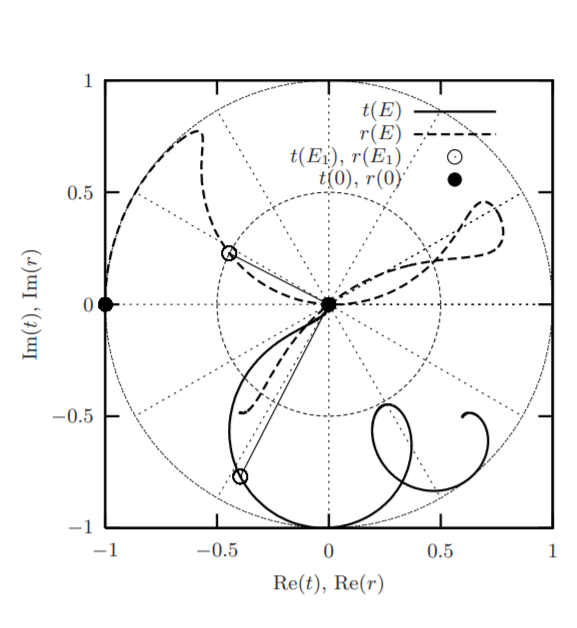
\includegraphics[scale=1]{3_21.PNG}
    \end{minipage}
    \begin{minipage}{0.5\textwidth}
        \captionsetup{font={Large}}
        \caption{Transmission ($t=\mid t\mid exp(i\bar{\delta})$) and reflection ($r=\mid r\mid exp(i\bar{\mathcal{X}})$) amplitudes for two repulsive $\delta$-functions at distance $w$. The plot starts at the energy $E = 0$ where $(t, r) = (0, -1)$ (black point) and runs through two resonances with $\mid t \mid = 1$. For $E\to\infty$, $t$ in turns approximates the value 1. The reflection amplitude r stands, according to $t^*r+r^*t=0$ perpendicular
        on $t$ (white dot). The phase $\mathcal{X}$
        jumps $\pm\pi$ at each resonance.}
    \end{minipage}
\end{figure}

\section{Periodic potentials}
We consider energy eigenstates in the periodic potential $V (x + w) = V (x)$, which are assumed to be constant in stucco, so that we can use the transfer matrix method, cf. Fig. 3.22. The Hamiltonian has the form
%公式 3.76
\begin{equation}
\begin{aligned} H &=\frac{p^{2}}{2 m}+V(x) \\ V(x+w) &=V(x) \text { periodic. } \end{aligned}
\end{equation}
The problem has the symmetry $V (x - w) = V (x)$, a discrete translation symmetry.
%图 3.22
\begin{figure}[ht]
    \begin{minipage}{0.5\textwidth}
        \centering
        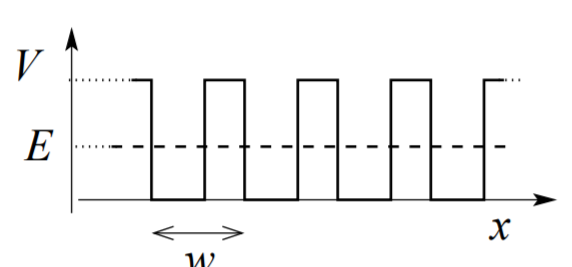
\includegraphics[scale=1]{3_22.PNG}
    \end{minipage}
    \begin{minipage}{0.5\textwidth}
        \captionsetup{font={Large}}
        \caption{Piece by piece constant, periodic potential $V (x) = V (x - w)$ with period $w$.}
    \end{minipage}
\end{figure}
We define the translation operator $T_w$ in place space by $T_{w}x = x + w$; Accordingly, there is a representation of $T_w$, the translation operator $U_w$, in the Hilbert space. He shifts wave functions accordingly
%公式 3.77
\begin{equation}
\begin{aligned}\left(U_{w} \Psi\right)(x) &=\Psi\left(T_{w}^{-1} x\right)=\Psi(x-w) \\\left\langle x | U_{w} \Psi\right\rangle &=\langle x-w | \Psi\rangle \end{aligned}
\end{equation}
both forms are equivalent, the second uses the Dirac notation. The translation around $w$ is a symmetry of the Hamiltonians, so interchange the operators, $HU_w = Uw_H$, or explicitly,
%公式 3.78
\begin{equation}
\begin{aligned}\left\langle x\left|H U_{w}\right| \Psi\right\rangle &=\left[-\left(\hbar^{2} / 2 m\right) \partial_{x}^{2}+V(x)\right]\left\langle x\left|U_{w}\right| \Psi\right\rangle \\ &=\left[-\left(\hbar^{2} / 2 m\right) \partial_{x}^{2}+V(x-w)\right]\langle x-w | \Psi\rangle \\ &=\langle x-w|H| \Psi\rangle=\left\langle x\left|U_{w} H\right| \Psi\right\rangle \end{aligned}
\end{equation}
This allows us to diagonalize $H$ and $U_w$ simultaneously,
%公式 3.79
\begin{equation}
\begin{aligned} H \Psi_{n k} &=E_{n k} \Psi_{n k} \\ U_{w} \Psi_{n k} &=\lambda_{k} \Psi_{n k} \end{aligned}
\end{equation}
We first look for the eigenvalues ​​$\lambda_k$. In doing so we require that the states are extended over the whole space, so the eigenvalue must have modulus 1 and can only be one phase, $\lambda_k = e^{-ikw}$; the associated quantum number $k$ defines the crystal momentum = $\hbar k$ (note that the crystal momentum is not equal to the particle momentum, since the translation symmetry is broken by the periodic potential, we can not expect a sharp momentum.) On the other hand, the continuous translation symmetry becomes the discrete symmetry the potential is replaced, and accordingly the crystal pulse replaces the usual pulse). The relation $exp [ikw] = exp [i (k + 2\pi n / w) w]$ allows us to limit the value range for the wave number k of the crystal momentum to $k \in [-\pi / w, \pi / w]$; the interval
%公式 3.80
\begin{equation}
    [-\pi / w, \pi / w] \quad \text { is called Brillouin zone. }
    \end{equation}
With
%公式 3.81
\begin{equation}
    \Psi_{n k}(x-w)=e^{-i k w} \Psi_{n k}(x) \quad \text { and } \quad \Psi_{n k}(x) \equiv e^{i k x} u_{n k}(x)
    \end{equation}
we get the periodic share
%公式 3.82
\begin{equation}
    u_{n k}(x-w)=u_{n k}(x) \quad \text { periodic. }
    \end{equation}
We find that $\Psi_{nk} (x)$ takes the form of a soft-modulated periodic function; $\Psi_{nk} (x)$ means (after Felix Bloch) Bloch wave function. The solutions of (3.76) are classified by two quantum numbers $n$ and $k$. We will see that $n$ is a band index (energy band) and $k$ describes the situation in the band. In the following we solve this\\\\
\textbf{Kronig-Penney model}\\\\
with the potential $V (x)$ given by a periodic sequence of $\delta$-functions, see Fig. 3.23
%公式 3.83
\begin{equation}
    V(x)=\sum_{n=-\infty}^{\infty} V_{0} \delta(x-n w)
    \end{equation}
We use the transfer matrix formalism around the context
%图 3.23
\begin{figure}[ht]
    \begin{minipage}{0.5\textwidth}
        \centering
        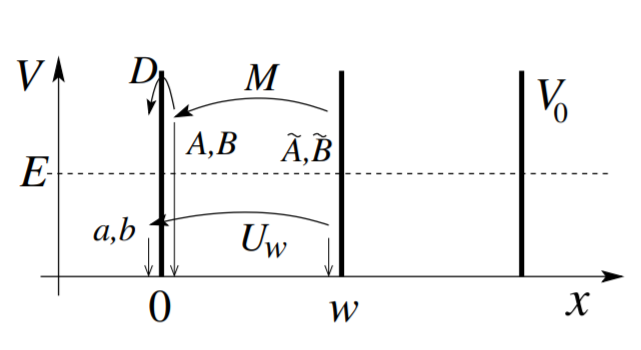
\includegraphics[scale=1]{3_23.PNG}
    \end{minipage}
    \begin{minipage}{0.5\textwidth}
        \captionsetup{font={Large}}
        \caption{Kronig-Penney Model: The periodic potential is defined as the sum of $\delta$-functions of the strong $V_0$ at a distance $w$.}
    \end{minipage}
\end{figure}
between the amplitudes $(a, b)$ and $(\tilde{A},\tilde{B})$ over a period, cf. see Fig. 3.23. With $v = mV_0 / \hbar^2$ and $E = \hbar^2K^2/2m$ (note that $K$ sets the energy while $k$ defines the crystal momentum) we find the relationships
%公式 3.84
\begin{equation}
\stackrel{(3.50)}{\longrightarrow}\left(\begin{array}{l}{a} \\ {b}\end{array}\right)=\left(\begin{array}{cc}{1+\frac{i v}{K}} & {\frac{i v}{K}} \\ {-\frac{i v}{K}} & {1-\frac{i v}{K}}\end{array}\right)\left(\begin{array}{l}{A} \\ {B}\end{array}\right)=D\left(\begin{array}{l}{A} \\ {B}\end{array}\right)\\
\stackrel{(3.10)}{\longrightarrow}\left(\begin{array}{l}{A} \\ {B}\end{array}\right)=\left(\begin{array}{cc}{\exp [-i K w]} & {0} \\ {0} & {\exp [i K w]}\end{array}\right)\left(\begin{array}{c}{\tilde{A}} \\ {\tilde{B}}\end{array}\right)=M\left(\begin{array}{c}{\tilde{A}} \\ {\tilde{B}}\end{array}\right)\\
\stackrel{(3.81)}{\longrightarrow}\left(\begin{array}{l}{a} \\ {b}\end{array}\right)=\left(\begin{array}{cc}{\exp [-i k w]} & {0} \\ {0} & {\exp [-i k w]}\end{array}\right)\left(\begin{array}{c}{\tilde{A}} \\ {\tilde{B}}\end{array}\right)=U_{w}\left(\begin{array}{c}{\tilde{A}} \\ {\tilde{B}}\end{array}\right)
\end{equation}
The comparison of the first two equations with the third gives the condition
%公式 3.85
\begin{equation}
\left(D M-U_{w}\right)\left(\begin{array}{c}{\tilde{A}} \\ {\tilde{B}}\end{array}\right)=0
\end{equation}
The existence of a non-vanishing wave requires that $\operatorname{det} (DM-U_w) = 0$, or simpler $\operatorname{det} (D-U_wM^{-1}) = 0$,
%
\begin{equation}
\begin{array}{c}{\operatorname{det}\left(\begin{array}{cc}{1+\frac{i v}{K}-e^{i(K w-k w)}} & {\frac{i v}{K}} \\ {-\frac{i v}{K}} & {1-\frac{i v}{K}-e^{-i(K w+k w)}}\end{array}\right)} \\ {=2 e^{-i k w}[\cos k w-\cos K w-(v / K) \sin K w]=0}\end{array}
\end{equation}
%图 3.24
\begin{figure}[ht]
    \begin{minipage}{0.5\textwidth}
        \centering
        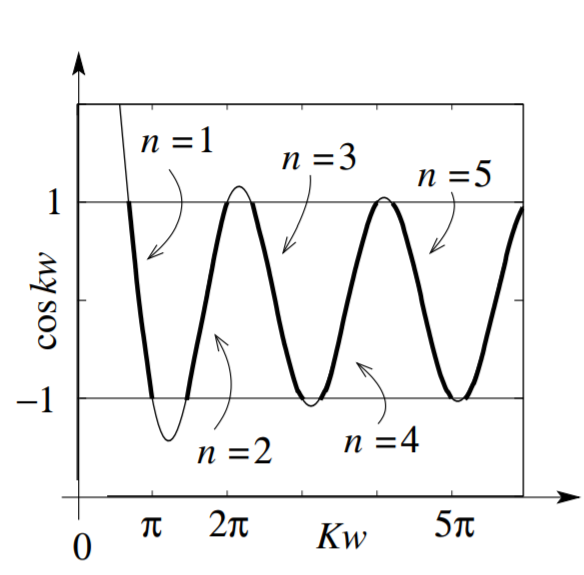
\includegraphics[scale=1]{3_24.PNG}
    \end{minipage}
    \begin{minipage}{0.5\textwidth}
        \captionsetup{font={Large}}
        \caption{Graphical representation of equation (3.87), $cos [k (K) w]$ vs $Kw$; Given $k$, determine $cos [kw] \in [-1, 1]$ and find the solution $K$. The solid lines enumerated by $n$ define the allowed values for $K$ from which the energy band $E_{nk}=\hbar^2K^2(n,k)/2m$.}
    \end{minipage}
\end{figure}
The implicit equation (compare Fig. 3.24)
%^公式 3.87
\begin{equation}
    \cos k w=\cos K w+v w \frac{\sin K w}{K w}
    \end{equation}
for given crystal moment $\hbar k \in [-\pi \hbar / w, \pi \hbar / w]$ determines the parameter $K$ and thus the energy
%公式 3.88
\begin{equation}
    E_{n k}=\frac{\hbar^{2}[K(n, k)]^{2}}{2 m}
    \end{equation}
%图 3.25
The solutions $K (k, n)$ arrange themselves in bands (indexed by $n$)
\begin{figure}[ht]
    \begin{minipage}{0.5\textwidth}
        \centering
        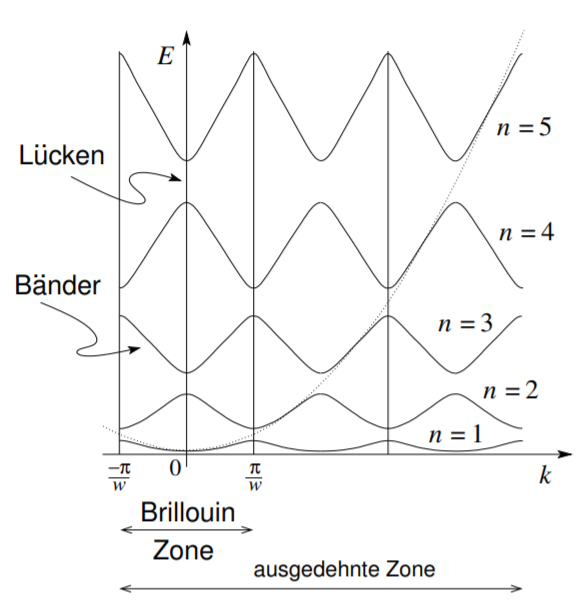
\includegraphics[scale=1]{3_25.PNG}
    \end{minipage}
    \begin{minipage}{0.5\textwidth}
        \captionsetup{font={Large}}
        \caption{Sketch of the energy band for a periodic potential. The quadratic dispersion $E(k)=\hbar^2k^2/2m$ (dotted line) of a free particle splits into allowed energy bands and forbidden energy lows. The crystal impulse $k$ is on the first Brillouin zone limited; the indices $n$ enumerate the bands. Alternatively, use the scheme with the periodically extended bands (avoid multiple counting).}
    \end{minipage}
\end{figure}
whence the allowed energies $E_{nk} = E (K (n, k)) = \hbar^2K^2 (n, k) / 2m$ and the forbidden areas that directly give up energy surges. Within the bands, the solutions are distinguished by the crystal impulse k, cf. see Fig. 3.25. Particles with energies in the band gaps are exponentially evaporated and can not propagate, for example, Tamm states on the surfaces of a crystal.
\section{Unordered $\text{potentials}^*$}
Unordered potentials create a new type of eigenstates localized in space (as opposed to the extended periodic potential Bloch waves). In the following we consider a piecewise constant random potential as shown in Fig. 3.26. Our analysis is different from the previous one. Instead of an eigenvalue problem to solve, we consider the transport of particles through the 'dirty ladder' = D-random potential. We calculate the resistance $R$ as a function of the length $L$ of the conductor and find that $R$ increases exponentially. We interpret this result as an exponential evaporation of the wave functions in the disorder potential.
%图 3.26
\begin{figure}[ht]
    \begin{minipage}{0.5\textwidth}
        \centering
        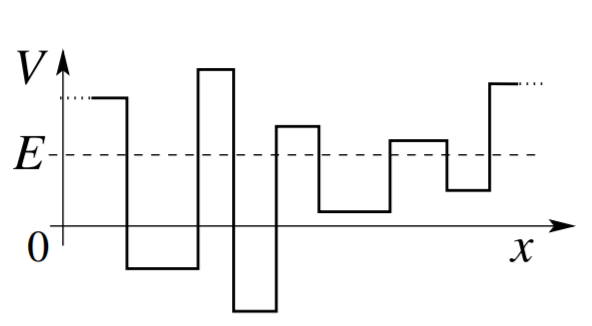
\includegraphics[scale=1]{3_26.PNG}
    \end{minipage}
    \begin{minipage}{0.5\textwidth}
        \captionsetup{font={Large}}
        \caption{Piecewise constant random potential.}
    \end{minipage}
\end{figure}
We first derive the Landauer formula for the transport of particles in one-dimensional conductive channels and calculate the resistance generated by a spreader. For this we consider the simplest case of a single barrier, cf. Figure 3.27.
%图 3.27
\begin{figure}[ht]
    \begin{minipage}{0.5\textwidth}
        \centering
        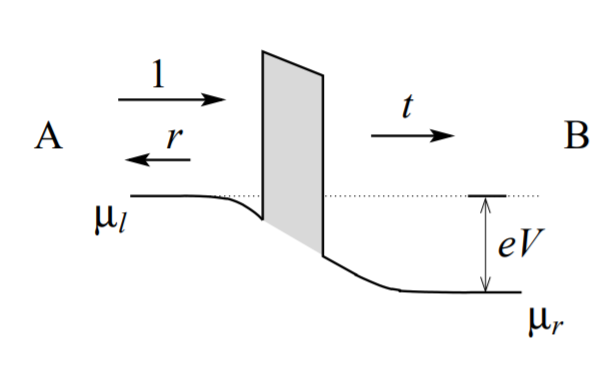
\includegraphics[scale=1]{3_27.PNG}
    \end{minipage}
    \begin{minipage}{0.5\textwidth}
        \captionsetup{font={Large}}
        \caption{Transport through a tunnel barrier which acts as a scattering center. The occupation levels (chemical potentials) $\mu_l,\mu)r$ of leads $A$ and $B$ differ by the established voltage $eV, \mu_l-\mu_r = eV$.}
    \end{minipage}
\end{figure}
The particles (electrons $e^-$) flow from line $A$ to line $B$; the reflection of the charged particles at the barrier creates an electric dipole that corresponds to a potential jump $V$ between the conductors. The potential shifts the bottom of the power straps so that the leads remain charge-neutral. Note that in this argument the current $I$
%图 3.28
\begin{figure}[ht]
    \begin{minipage}{0.5\textwidth}
        \centering
        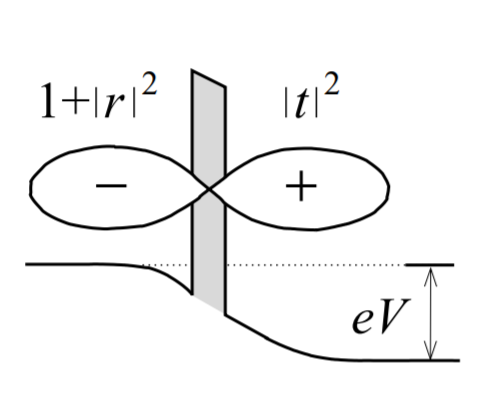
\includegraphics[scale=1]{3_28.PNG}
    \end{minipage}
    \begin{minipage}{0.5\textwidth}
        \captionsetup{font={Large}}
        \caption{Landauer dipole: Reflected electrons accumulate in front of the barrier and generate a negative excess charge; these are missing on the jerky side of the spreader resulting in an uncompensated positive charge. The resulting charge dipole is ultimately compensated by the applied voltage.}
    \end{minipage}
\end{figure}
the driver is and the potential $V$ defines the answer. Let $I_0$ be the incident current, then the current $I = I_0 | t |^2$ is transported from $A$ to $B$. The dipole to be compensated involves the charge density
%公式 3.89
\begin{equation}
\begin{aligned} \delta n &=n_{l}-n_{r}=\frac{I_{0}}{e v}\left(1+|r|^{2}-|t|^{2}\right) \\ v &=\partial E / \partial p \quad \text { the speed. } \end{aligned}
\end{equation}
This charge density is compensated by a corresponding charge density, which results from the displacement of the bands in the supply lines around the potential $V$ results,
%公式 3.90
\begin{equation}
    \begin{split}
        \delta n=\left.\frac{1}{L} \frac{d N}{d E}\right|_{\text {Total }} e V & \text{ with} \quad \frac{d E}{d N}=\frac{d E}{d k} \frac{d k}{d N}=\hbar v \frac{2 \pi}{L}\\
        &\text { and }\left.\quad \frac{d N}{d E}\right|_{\text {Total }}=\frac{d N}{d E} \underbrace{\cdot 2}_{\text {Spin}}\underbrace{\cdot 2}_{direction}\\   
    \end{split}
\end{equation}
For the resistance $R = V / I$ we find the result
%公式 3.91
\begin{equation}
    R=\frac{I_{0}\left(1+|r|^{2}-|t|^{2}\right) h v}{4 e v e I_{0}|t|^{2}}=\frac{h}{2 e^{2}} \frac{|r|^{2}}{|t|^{2}}
    \end{equation}
where the quantum resistance is the universal value
%公式 3.92
\begin{equation}
    R_{Q}=R_{K}=h / e^{2} \cong 25.812807449 \mathrm{k} \Omega
    \end{equation}
accepts (a Klitzing). The size (If the voltage across the reservoirs (instead of the lines) is measured, then to the resistance $R_Q | r |^2/2|t|^2$ for each contact between reservoir and conductor a contact resistance (Sharvin resistance) $R_Q / 4$ to add, so $R = (R_Q / 2) (| r |^2/|t|^2+2\cdot 1/2=R_Q/2|t|^2$ resulting in a conductance $G = (2e^2/h)\mid t\mid^2$ between the reservoirs.)

%公式 3.93
\begin{equation}
    G=1 / R=\frac{2 e^{2}}{h} \frac{|t|^{2}}{|r|^{2}}
    \end{equation}
is called conductance, $I = G · V$.
We next consider the resistance of a disordered conductor, i. Let $V (x)$ be a disordered, piecewise constant potential. We start with an incident amplitude 1 and want to calculate the transmission $t$, see Figure 3.29,

%图 3.29
\begin{figure}[ht]
    \begin{minipage}{0.5\textwidth}
        \centering
        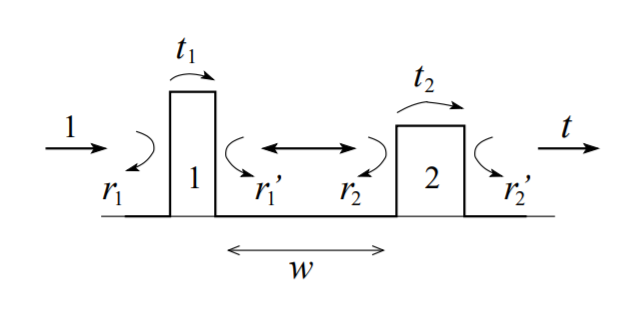
\includegraphics[scale=1]{3_29.PNG}
    \end{minipage}
    \begin{minipage}{0.5\textwidth}
        \captionsetup{font={Large}}
        \caption{Stuckwise constant potential with two barriers. For the transmission through the whole structure, all paths with multiple reflections are to be considered.}
    \end{minipage}
\end{figure}
%公式 3.94
\begin{equation}
\begin{aligned} t &=t_{1} t_{2}+t_{1} r_{2} r_{1}^{\prime} t_{2}+t_{1} r_{2} r_{1}^{\prime} r_{2} r_{1}^{\prime} t_{2}+\cdots \\ &=t_{1} \frac{1}{1-r_{2} r_{1}^{\prime}} t_{2} \end{aligned}
\end{equation}
The resistance ($[R]$ in units $h / 2e^2$) over the reservoirs is
%公式 3.95
\begin{equation}
    R=1 /|t|^{2}-1=\left|1-r_{2} r_{1}^{\prime}\right|^{2} /\left|t_{1}\right|^{2}\left|t_{2}\right|^{2}-1
    \end{equation}
We average over the distance $w$, then the term $\langle r_2 r_1^{\prime}\rangle_w=0$ does not contribute because the coefficients contain random phases $e^{ikw}$ and we find
%公式 3.96
\begin{equation}
\begin{aligned} R=\frac{1+\left|r_{2}\right|^{2}\left|r_{1}^{\prime}\right|^{2}}{\left|t_{1}\right|^{2} | r_{2}^{\prime}}-1 &=\left(\frac{1}{\left|t_{1}\right|^{2}}-1\right)+\left(\frac{1}{\left|t_{2}\right|^{2}}-1\right) \\ &+2\left(\frac{1}{\left|t_{1}\right|^{2}}-1\right)\left(\frac{1}{\left|t_{2}\right|^{2}}-1\right) \\ &=\underbrace{R_{1}+R_{2}}_{\text {classical result }}+\underbrace{2 R_{1} R_{2}}_{\text {qm-interference }} \end{aligned}
\end{equation}
The interference term has a drastic effect on the result in that the resistance $R$ increases exponentially with the length. We show this by extending a disordered ladder stub of Lange $L$ by one piece $dL$ and calculating the increase in resistance. We set $R_1 = R (L), R_2 = dR = \alpha dL$, the small addition. Then

%公式 3.97
\begin{equation}
\begin{aligned} R(L+d L) &=R(L)+\underbrace{\alpha d L}_{d R}+2 \alpha R d L \quad \alpha=\partial_{L} R \\ \Rightarrow \partial_{L} R &=\alpha(\underbrace{1}_{\text {classical }}+\underbrace{2 R}_{\mathrm{qm}}) \end{aligned}
\end{equation}
The classical term alone yields a result linear in $L, R (L) = \alpha L$. Taking into account the quantum mechanical interferences results in an exponential increase of the resistance
%公式 3.98
\begin{equation}
\begin{aligned} \ln \frac{1+2 R}{1+2 R_{0}} &=2 \alpha\left(L-L_{0}\right) \\ \overset{R_{0} \text { small }}{\to} & \approx\left(e^{2 \alpha L}-1\right) / 2 \end{aligned}
\end{equation}
We interpret this result as meaning that the states are localized in the disordered potential, that is, the wave functions are eliminated due to destructive interference and decay exponentially with the distance $L, \Psi \propto exp (-\alpha x)$ and therefore $R \propto exp (2\alpha x)$.

\subsection{Comparison $V (x)$ periodic $\leftrightarrow V (x)$ disordered}
As well as in the periodic as well as in the disordered potential, interferences play an important role, see Fig. 3.30. At the periodic potential, these interferences are regular and either constructive when the energy is within an allowable energy band or destructive when the energy is placed in a forbidden gap. Positive interferences result in modulated periodic Bloch functions of infinite extent. \\\\
In the random potential the positive interferences appear only locally,
%图 3.30
\begin{figure}[ht]
        \centering
        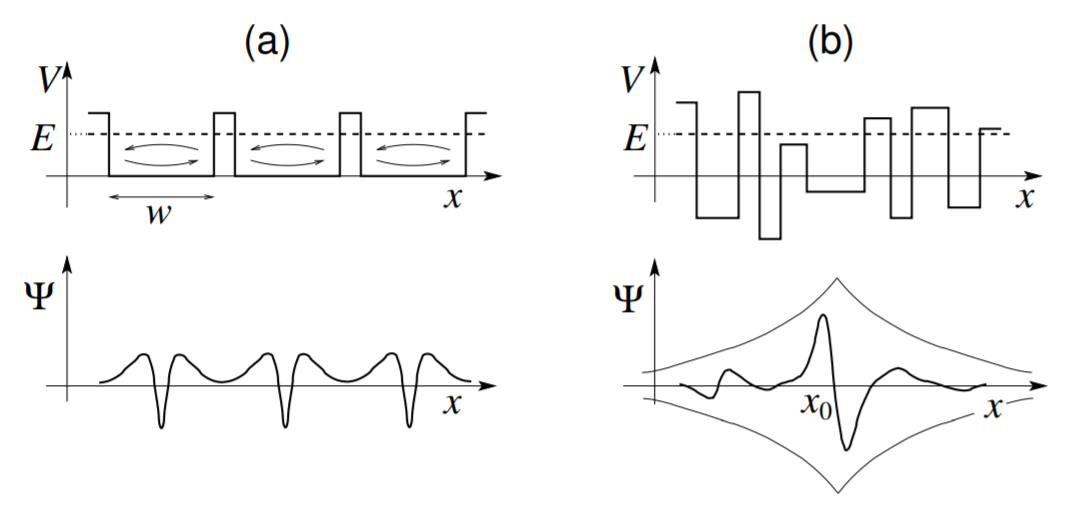
\includegraphics[scale=1]{3_30.PNG}
        \captionsetup{font={Large}}
        \caption{Wave functions in the periodic (a) and in the random potential (b). Constructive interferences in the periodic potential produce extended Bloch functions. In the disordered potential, constructive interferences arise only locally (depending on E) and the wave functions decompose exponentially $\propto exp[-\alpha(E)\mid x-x_0(E)\mid]$.}
\end{figure}
constructive interference over long distances is never possible. Dependent on the energy and the details of the potential arise localized eigenfunctions which decompose exponentially; whose center 'jumps' with the change of $E$.
In dim = 1, all states in the $V_{coincidence}(x)$ are exponentially localized. In dim = 3 there is a bounded energy $E_M$ (index $M$ for 'mobility') which separates extended from localized states. The situation for dim = 2 is marginal, that is, all states are just localized.
For hackers: Solve the problem $V (x)$ -periodic and unordered using the transfermatrix technique on the computer. Select $V$ in a staggering way. For the disordered case, it is sufficient to choose the positions $x_i$ by chance. More details can be found in the article by Anderson, Thouless, Abrahams, Fisher, Phys. Rev. B 22, 3519 (1980).
\section{Harmonic oscillator}
The harmonic oscillator is a 'Drosophila' of quantum mechanics. Many problems can be traced back to the (shifted) harmonic oscillator and thus become exactly soluble (phonons in the crystal lattice, $e^-$ in the magnetic field, $H_{c2}$ in the type II superconductor, electromagnetic radiation field, · · ·). A detailed discussion is coming up. We define the problem via the Hamiltonian H with the potential $V (q) = (f / 2) q^2$ (see Fig. 3.31),
%公式 3.99
%公式 3.99
\begin{equation}
    \begin{split}{l} 
        &\quad H =\frac{p^{2}}{2 m}+\frac{f}{2} q^{2} \\ 
        &\quad \overset{\omega^{2} =\frac{f}{m}}{=}  \frac{p^{2}}{2 m}+\frac{1}{2} m \omega^{2} q^{2} \\
        &[p, q] =\hbar / i \quad \rightarrow \quad p=-i \hbar \partial_{q} 
    \end{split}
    \end{equation}
We are looking for the stationary states with $H\Psi = E\Psi$ and boundary conditions $\Psi(q\to\pm\infty)=0$. We go over to dimensionless variables,
%公式 3100
\begin{equation}
\begin{aligned} x=\sqrt{\frac{m \omega}{\hbar}} q \rightarrow q &=\sqrt{\frac{\hbar}{m \omega}} x \\ p &=-i \sqrt{m \hbar \omega} \partial_{x} \\ H &=\frac{\hbar \omega}{2}\left(-\partial_{x}^{2}+x^{2}\right), \quad\left[i \partial_{x}, x\right]=i \end{aligned}
\end{equation}
%图 3.31
\begin{figure}[ht]
    \begin{minipage}{0.5\textwidth}
        \centering
        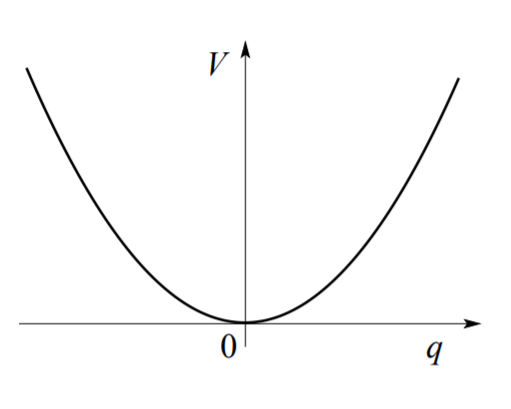
\includegraphics[scale=1]{3_31.PNG}
    \end{minipage}
    \begin{minipage}{0.5\textwidth}
        \captionsetup{font={Large}}
        \caption{Harmonic potential $V(q)=fq^2/2=mw^2q^2/2 \text{ with }w=\sqrt{f/m}$.}
    \end{minipage}
\end{figure}
It is
%公式 3101
\begin{equation}
\begin{aligned} \hbar \omega=\hbar \sqrt{f / m}, &[f]=F / L=E / L^{2} \quad \text { the spring constant } \\ &[f / m]=E / m L^{2}=\sec ^{-2} \Rightarrow \hbar \omega \text { an energy. } \end{aligned}
\end{equation}
We obtain the eigenvalue problem $H\Psi=E\Psi$ in the dimensionless form
%公式 3102
\begin{equation}
    \left[\partial_{x}^{2}+\lambda-x^{2}\right] \Psi=0, \quad \lambda=\frac{2 E}{\hbar \omega}
    \end{equation}
This problem can be solved in various ways.
3.10.1 Conventional solution
The leading term for $x \to \infty \text{ is } (x^2 \gg \lambda)$,
%公式 3103
\begin{equation}
    \left(\partial_{x}^{2}-x^{2}\right) \Psi=0 \quad \rightarrow \quad \Psi \propto e^{-x^{2} / 2}
    \end{equation}
($\partial_x\Psi=-x\Psi,\partial_x^2\Psi=-\Psi+x^2\Psi\approx x^2\Psi$ for $x\to\infty$). We use the approach $\Psi(x)=H(x)e^{-x^2/2}$ and find the differential equation for $H(x)$,
%公式 3104
\begin{equation}
    \left[\partial_{x}^{2}-2 x \partial_{x}+(\lambda-1)\right] \mathrm{H}(x)=0
    \end{equation}
We use the Fuchs approach for the solution
%公式 3105
\begin{equation}
    \mathrm{H}(x)=x^{s} \sum_{n} a_{n} x^{n}
    \end{equation}
with $a0 \neq 0$ and $s \geq 0$, and find by coefficient comparison
%公式 3106
\begin{equation}
\begin{aligned} s(s-1) a_{0} &=0 \\(s+1) s a_{1} &=0 \\(s+2)(s+1)a_2-(2s+1-\lambda) a_{0} &=0 \\ \vdots &  \\(s+n+2)(s+n+1) a_{n+2}-(2 s+2 n+1-\lambda) a_{n} &=0 \end{aligned}
\end{equation}
By assumption, $a0 \neq 0$, which is why $s = 0$ or $s = 1$; Furthermore, without limiting generality, we set $a_1 = 0$. From these
Conditions arise
\begin{itemize}
    \item[-]  for $s = 0, H (x) = a_0 + a_2x
    ^2 + \cdots$ even in $x$,
    \item[-]  for $s = 1, H (x) = x (a_0 + a_2x
    ^2 + \cdots)$ odd in $x$.
\end{itemize}
Note that $ V (q) = V (-q)$ and thus $[P, H] = 0$, which means that we can find eigenfunctions with defined parity. The asymptotic $a_{n + 2} / a_n \to 2 / n$ yields (at least) an asymptotic behavior $H \sim exp (x^2) \text{ for } x\to\infty,$ so the series for $H (x)$ overcompensates for the asymptotic $\sim exp (-x^2 / 2)$ in the approach $\Psi (x ) = H (x) e^{-x^ 2/2}$ The boundary condition $lim_{x \to\infty}\Psi (x) \to 0$ can only be satisfied if the series breaks off and we obtain the eigenvalues $​​λ_n = 2n + 1$ with eigenfunctions $\Psi_n = H_n (x ) exp (-x^2 / 2)$, $Hn (x)$ the Hermite polynomial in summary we find the result

%公式 3107
\begin{equation}
\begin{aligned}
&\left\{\begin{array}{cl}{\lambda_{n}=} & {2n+1} \\ {\Psi_{n}=} & {N_{n} \mathrm{H}_{n}(x) \exp \left[-x^{2} / 2\right]} \\ {0=} & {\mathrm{H}_{n}^{\prime \prime}-2 x \mathrm{H}_{n}^{\prime}+2 n \mathrm{H}_{n}}\\ & \mathrm{H}_{0}=1, \quad \mathrm{H}_{1}=2 x \\ & \mathrm{H}_{2}=4 x^{2}-2, \cdots \\ & N_{0}=1 / \pi^{1 / 4}, N_{n}=N_{0} / \sqrt{2^{n} n !} \\ E_{n}=& \hbar \omega\left(\frac{1}{2}+n\right) 
\end{array}\right.
\end{aligned}
\end{equation}
Note that $q = \sqrt{\hbar/mwx} , \to N_0=\sqrt[4]{mw/\pi\hbar}$ in the q coordinate. This solution path represents the standard procedure: Separate the asymptotic ($e^{-x^2/2}$) for$ x \to\infty$, find the correction (here the function $H (x)$) through a series approach; the boundary condition (RB) demands the discontinuation of the series and the spectrum $E_n$ and the polynomial portions of the eigenfunctions $\propto H_n$ are obtained. In the following we consider a more elegant way.
\subsection{Elegant solution}
This is based on an operator technique with ascending and descending operators as used for the second quantization. We define
%公式 3108
\begin{equation}
\begin{aligned} a & \equiv \frac{1}{\sqrt{2}}\left(x+\partial_{x}\right)=\frac{1}{\sqrt{2}}\left(\sqrt{\frac{m \omega}{\hbar}} q+\frac{i}{\sqrt{m \hbar \omega}} p\right) \\ a^{\dagger} & \equiv \frac{1}{\sqrt{2}}\left(x-\partial_{x}\right) \end{aligned}
\end{equation}
is reversed
%公式 3109
\begin{equation}
\begin{aligned} x &=\frac{1}{\sqrt{2}}\left(a+a^{\dagger}\right) \\ \partial_{x} &=\frac{1}{\sqrt{2}}\left(a-a^{\dagger}\right) \end{aligned}
\end{equation}
Substituting in (3.100) yields the Hamiltonian
%公式 3110
\begin{equation}
\begin{aligned} H &=\frac{\hbar \omega}{2}\left(-\partial_{x}^{2}+x^{2}\right) \\ &=\frac{\hbar \omega}{4}\left[-\left(a-a^{\dagger}\right)\left(a-a^{\dagger}\right)+\left(a+a^{\dagger}\right)\left(a+a^{\dagger}\right)\right] \\ &=\frac{\hbar \omega}{4}\left(-a^{2}+a a^{\dagger}+a^{\dagger} a-a^{\dagger 2}+a^{2}+a a^{\dagger}+a^{\dagger} a+a^{\dagger 2}\right) \\ &=\hbar \omega\left(a^{\dagger} a-\left[a^{\dagger}, a\right] / 2\right) \end{aligned}
\end{equation}
For the commutator we find (compare (3.100))
%公式 3111
\begin{equation}
\begin{aligned}\left[a, a^{\dagger}\right] &=\frac{1}{2}\left[\left(x+\partial_{x}\right)\left(x-\partial_{x}\right)-\left(x-\partial_{x}\right)\left(x+\partial_{x}\right)\right] \\ &=\frac{1}{2}\left(-x \partial_{x}+\partial_{x} x\right) 2=1 \end{aligned}
\end{equation}
We define the operator $N = a^{\dagger} a$ such that
%公式 3112
\begin{equation}
    H=\hbar \omega\left(N+\frac{1}{2}\right)
    \end{equation}
The eigenvalue problem $H\Psi = E\Psi$ reduces too
%公式 3113
\begin{equation}
    N|n\rangle= n|n\rangle
    \end{equation}
which leads us to diracnotation, $|n\rangle\leftrightarrow\Psi_n$. We investigate the effect of the operators $a^{\dagger}$ and a on the eigenstates $\langle n\rangle$ of N. For this we determine the commutators of $N$ with $a^{\dagger}$ and with $a$,
%公式 3114
\begin{equation}
    \left[N, a^{\dagger}\right]=\left[a^{\dagger} a, a^{\dagger}\right]=a^{\dagger}\left[a, a^{\dagger}\right]+\left[a^{\dagger}, a^{\dagger}\right] a=a^{\dagger}
    \end{equation}
%公式 3115
\begin{equation}
    [N, a]=\left[a^{\dagger} a, a\right]=a^{\dagger}[a, a]+\left[a^{\dagger}, a\right] a=-a
    \end{equation}
The conditions
%公式 3116
\begin{equation}
    a^{\dagger}|n\rangle, \quad a|n\rangle
    \end{equation}
then define new eigenvectors to $N$ with eigenvalue $n + 1$ and $n - 1$:
%公式 3117
\begin{equation}
\begin{aligned} N a^{\dagger}|n\rangle &=\left(a^{\dagger} N+\left[N, a^{\dagger}\right]\right)|n\rangle= a^{\dagger} n|n\rangle+ a^{\dagger}|n\rangle=(n+1) a^{\dagger}|n\rangle \\ N a|n\rangle &=(a N+[N, a])|n\rangle= a n|n\rangle- a|n\rangle=(n-1) a|n\rangle \end{aligned}
\end{equation}
The operators $a^{\dagger}$ and a thus increase and decrease the eigenvalue n of an eigenstate $\langle n\rangle$ by 1; this property is a consequence of the commutation relations between $a, a^{\dagger}$, and $N = a^{\dagger} a$ (which ultimately defines the spectrum),
%公式 3118
\begin{equation}
    \left[a, a^{\dagger}\right]=1, \quad\left[N, a^{\dagger}\right]=a^{\dagger}, \quad[N, a]=-a
    \end{equation}
We call $a^{\dagger}$ an ascending operator and $a$ descending operator. The states $a^{\dagger}\langle n\rangle$ and $a\langle n\rangle$ are not yet normalized: Let $\langle n|n\rangle = 1$ be normalized, then
%公式 3119
\begin{equation}
\begin{aligned}\left\langle n\left|a^{\dagger} a\right| n\right\rangle &=\langle n|N| n\rangle= n \text { and } \\\left\langle n\left|a a^{\dagger}\right| n\right\rangle &=\left\langle n\left|\left[a, a^{\dagger}\right]+a^{\dagger} a\right| n\right\rangle= n+1 \end{aligned}
\end{equation}
and we get normalized eigenvectors when we define
%公式 3120
\begin{equation}
\begin{aligned}|n-1\rangle &=\frac{1}{\sqrt{n}} a|n\rangle \\|n+1\rangle &=\frac{1}{\sqrt{n+1}} a^{\dagger}|n\rangle \end{aligned}
\end{equation}
In the next step we determine the eigenvalues ​​n via an abort criterion. Let $|n\rangle$ be an eigenvector of eigenvalue $n$, then
%公式 3121
\begin{equation}
    a^{k}|n\rangle=\sqrt{n(n-1)(n-2) \cdots(n-k+1)}|n-k\rangle
    \end{equation}
and $|n-k\rangle$ is an eigenvector to eigenvalue $n - k$. But we have $n = \langle n | N | n\rangle = \langle an | an\rangle \geq 0$. If we choose $k \in\mathbb{N}$ big enough we get a negative eigenvalue $n - k$ to $N \Rightarrow$  the iteration has to be aborted and so $n$ has to be integer $\geq 0$ be. The smallest eigenvalue is $n = 0$ and
%公式 3122
\begin{equation}
    a|0\rangle= 0
    \end{equation}
i.e. the operator annihilates $|0\rangle$. Then all $|n\rangle$ are followed by applying $a^{\dagger}$,
%公式 3123
\begin{equation}
    |n\rangle=\frac{\left(a^{\dagger}\right)^{n}}{\sqrt{n !}}|0\rangle, \quad n \geq 0
    \end{equation}
The eigenvalue $n$ determines the energy
%公式 3124
\begin{equation}
    E_{n}=\hbar \omega\left(N+\frac{1}{2}\right)=\hbar \omega\left(n+\frac{1}{2}\right)
    \end{equation}
thus $n$ counts the existing energy quantum $\hbar w$. The application of $a^{\dagger}$ generates an additional quantum of energy that increases the oscillation amplitude of the oscillator. The lowest eigenstate, the ground state $|0\rangle$, has no energy quanta, but a finite energy $E_0 = \hbar ω / 2 \neq 0$, a consequence of Heisenberg's uncertainty principle (HUP): the particle can not stay sharp at $x = 0 \Rightarrow$ the uncertainty makes the expectation $\langle H\rangle \neq 0$ finite, even in the ground state; the energy $\hbar w/2$ is the result of the zero point vibrations (of the vacuum). We can easily estimate this minimal energy: the HUP implies $\delta p\sim \hbar/\delta x$, thus $E \backsimeq \hbar^2/ 2m\delta x^2 + mω^2 \delta x^2 / 2$; $E$ is minimal for $E_{pot}\sim E_{kin}\to\delta x \sim \sqrt{\hbar/ mω}$ and $E \sim \hbar ω.$ The numerical factor 1/2 results from the exact calculation.
We call:
%公式 3125
\begin{equation}
\begin{aligned} 
    &a  \qquad \text { the drop-off or destruction operator, } \\ 
    &a^{\dagger} \,\,\,\quad\text { the ascending or generating operator, } \\ 
    & \qquad\qquad\quad \uparrow \text { in } n \qquad\quad\uparrow\text{of energy quanta}\\
    &|0\rangle= \text { the ground state or the vacuum } \\ 
    & \qquad\qquad\quad  \uparrow \text { in } n\qquad\quad\uparrow \text{ no quanta.} \\ 
    &N= \text { Pay the quanta in the system. } \end{aligned}
\end{equation}
We can interpret the quanta as 'particles' of energy $\hbar w$, then have
%公式 3126
\begin{equation}
\begin{array}{l}{|0\rangle=\text { the vacuum }=\text { no 'particles' }} \\ {|n\rangle= n \text { energy quanta }=n \text { n 'particles'. }}\end{array}
\end{equation}
Finally, we still need the wave functions, first $| 0\rangle$, the vacuum. It is $a | 0\rangle = 0$, in place representation, (Note the drop $\propto exp (-x^2 / 2)$ when the wave function enters the forbidden zone, compare this to a potential step and with a linear potential, Eq (3.161))
%公式 3127
\begin{equation}
\begin{aligned} 0=\sqrt{2}\langle x|a| 0\rangle=&\left(x+\partial_{x}\right)\langle x | 0\rangle=\left(x+\partial_{x}\right) \Psi_{0}(x) \\ \Rightarrow &\langle x | 0\rangle \propto e^{-x^{2} / 2} \\ & \downarrow \text { Normierung } \\ &\langle x | 0\rangle=\frac{1}{\sqrt[4]{\pi}} e^{-x^{2} / 2} \end{aligned}
\end{equation}
The states $\langle x | n\rangle$ follow by iterative application of $a^{\dagger}$,
%公式 3128
\begin{equation}
\begin{aligned}\langle x | 1\rangle=\left\langle x\left|a^{\dagger}\right| 0\right\rangle &=\frac{1}{\sqrt{2}}\left(x-\partial_{x}\right) \frac{1}{\sqrt[4]{\pi}} e^{-x^{2} / 2}=\frac{1}{\sqrt{2 \sqrt{\pi}}} 2 x e^{-x^{2} / 2} \\ &=\sqrt{\frac{2}{\sqrt{\pi}}} x e^{-x^{2} / 2} \\\langle x | n\rangle &=\frac{1}{\sqrt{2^{n} n ! \sqrt{\pi}}}\left(x-\partial_{x}\right)^{n} e^{-x^{2} / 2} \\ &=\frac{1}{\sqrt{2^{n} n ! \sqrt{\pi}}} \mathrm{H}_{n}(x) e^{-x^{2} / 2} \end{aligned}
\end{equation}
With
%公式 3129
\begin{equation}
\begin{array}{l}{\mathrm{H}_{0}=1} \\ {\mathrm{H}_{1}=2 x} \\ {\mathrm{H}_{2}=(2 x)^{2}-2} \\ {\mathrm{H}_{3}=(2 x)^{3}-6(2 x)} \\ {\mathrm{H}_{4}=(2 x)^{4}-12\left(2 x^{2}\right)+12}\end{array}
\end{equation}
The form of eigenfunctions is given in Figure 3.32. Going over to the variable variable $q = \sqrt{\hbar/ mω} x$ we ​​obtain
%公式 3130
\begin{equation}
    \langle q | n\rangle=\sqrt{\sqrt{\frac{m \omega}{\pi \hbar}} \frac{1}{2^{n} n !}} \mathrm{H}_{n}(\sqrt{m \omega / \hbar} q) e^{-\left(m \omega q^{2}\right) / 2 \hbar}
    \end{equation}

%图 3:32
\begin{figure}[ht]
        \centering
        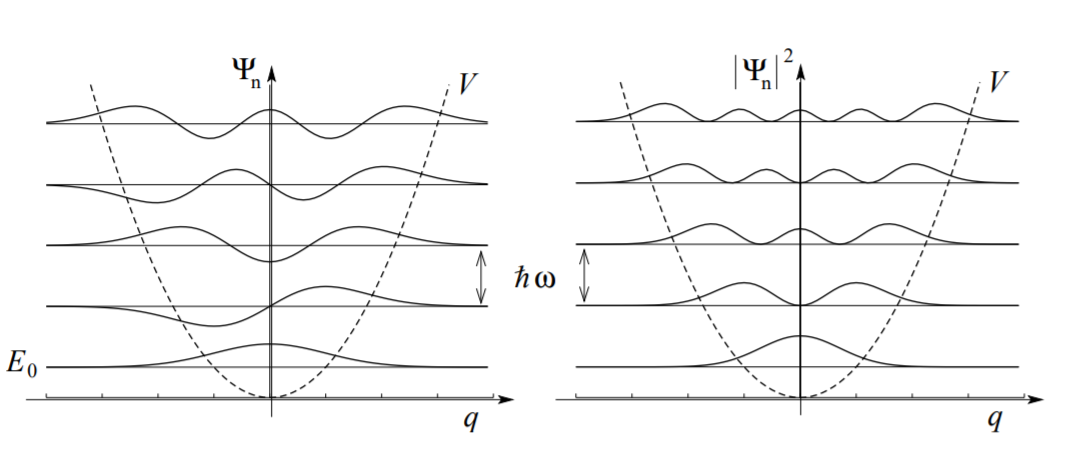
\includegraphics[scale=1]{3_32.PNG}
        \captionsetup{font={Large}}
        \caption{Eigenfunctions ($\propto$ Hermite polynomials) of the harmonic oscillator, on the left the amplitudes $\Psi_n$, on the right the probabilities $\mid \Psi_n\mid$}
\end{figure}
\subsection{Classic Limes}
For large energies $E_n$, the quantum mechanical solution approaches the classic $\to$ classical Limes. The classical probability of residence and energy are given by ($W_{kl}dx = dt / T$)
%公式 3131
\begin{equation}
\begin{aligned} W_{\mathrm{kl}} &=\frac{1}{2 \pi q_{0} \sqrt{1-\left(x / q_{0}\right)^{2}}} \\ E_{\mathrm{kl}} &=\frac{1}{2} m \omega^{2} q_{0}^{2} \end{aligned}
\end{equation}
In Figure 3.33 we compare this classical result with the quantum mechanical for $n=10$ quanta, where the amplitude $q_0$ is given by $E_{kl} = E_{10}$.
%图 3:33
\begin{figure}[ht]
    \begin{minipage}{0.5\textwidth}
        \centering
        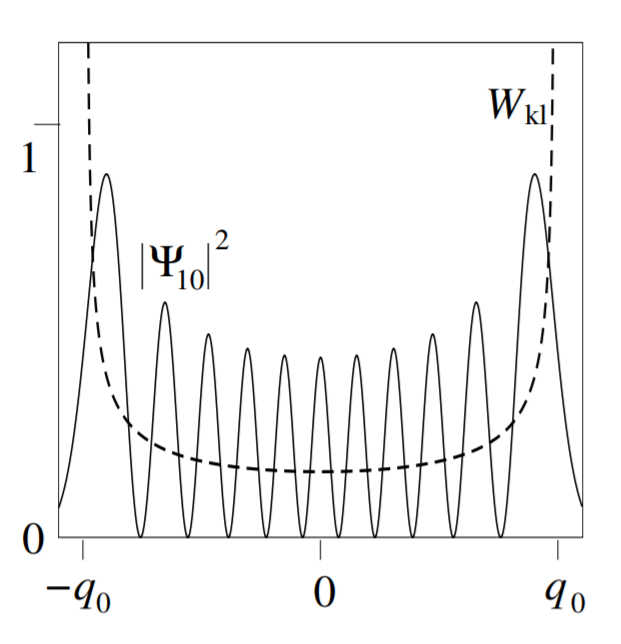
\includegraphics[scale=1]{3_33.PNG}
    \end{minipage}
    \begin{minipage}{0.5\textwidth}
        \captionsetup{font={Large}}
        \caption{Classic Limes of the harmonic Oscillator. The probability $\mid\Psi_{10}\mid^2$ approximates (after averaging over small scales) the classical result $W_{kl}(q_0)$, where $q_0$ follows from the relation $E_{kl} = E_{10}$ between the energies.}
    \end{minipage}
\end{figure}
\subsection{Coherent States}
Coherent states are eigenstates of the annihilation operator $a$,
%公式 3132
\begin{equation}
    a|\alpha\rangle=\alpha|\alpha\rangle
    \end{equation}
With $a|n\rangle=\sqrt{n}|n-1\rangle$, cf. (3.120), one easily finds that the series
%公式 3133
\begin{equation}
    |\alpha\rangle= e^{-|\alpha|^{2} / 2} \sum_{n=0}^{\infty} \frac{\alpha^{n}}{\sqrt{n !}}|n\rangle
    \end{equation}
the eigenvalue problem (3.132) with $\alpha \in\mathbb{C}$ arbitrary, solving. The time evolution of the coherent states has the form
%公式 3134
\begin{equation}
    |\alpha\rangle(t)=|\alpha(t)\rangle e^{-i \omega t / 2} \operatorname{mit} \alpha(t)=\alpha e^{-i \omega t}
    \end{equation}
and produces the amplitude of a classical vibration,
%公式 3135
\begin{equation}
    \langle x\rangle_{\alpha}(t)=\sqrt{\hbar / 2 m \omega}\left[\alpha(t)+\alpha^{*}(t)\right]
    \end{equation}
Coherent states are of great importance in quantum optics. Further details in the exercises.
\section{Morse potential}
The Morse potential
%公式 3136
\begin{equation}
    V(x)=V_{0}\left(e^{-2 x / x_{0}}-2 e^{-x / x_{0}}\right)
    \end{equation}
is sketched in Fig. 3.34. As usual, we solve the eigenvalue problem
%图 3:34
\begin{figure}[ht]
    \begin{minipage}{0.5\textwidth}
        \centering
        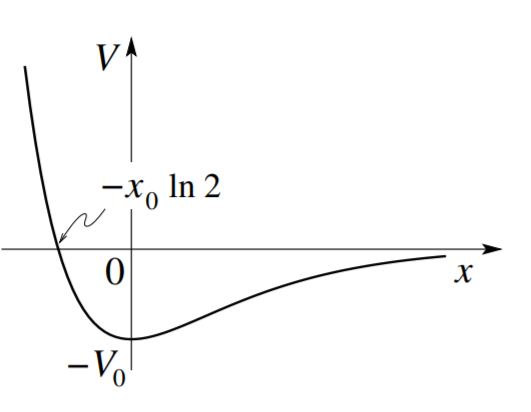
\includegraphics[scale=1]{3_34.PNG}
    \end{minipage}
    \begin{minipage}{0.5\textwidth}
        \captionsetup{font={Large}}
        \caption{Morse potential $V (x) = V_0 [exp (-2x / x_0) - 2 exp (-x / x_0)]$; the half-sided potential with repulsive and attractive portions is suitable for describing a surface. Note the exponential behavior compared to the algebraic Lennard-Jones (particle-particle) potential $V(r)=4V_0[(r_0/r)^{12}-(r_0/r)^6]$.}
    \end{minipage}
\end{figure}
%公式 3137
\begin{equation}
    H \Psi=E \Psi
    \end{equation}
for $E <0 (E> 0)$ we obtain a discrete (continuous) spectrum. To the solution of
%公式 3138
\begin{equation}
    \left[-\frac{\hbar^{2}}{2 m} \partial_{x}^{2}+V_{0}\left(e^{-2 x / x_{0}}-2 e^{-x / x_{0}}\right)-E\right] \Psi=0
    \end{equation}
let's go over to new variables,
%公式 3139
\begin{equation}
\begin{aligned} k_{0} &=& \frac{1}{\hbar} \sqrt{2 m V_{0}}, & y=2 k_{0} x_{0} e^{-x / x_{0}} \\ \alpha &=\frac{1}{\hbar} \sqrt{2 m|E|}, & e &=\alpha x_{0} \end{aligned}
\end{equation}
and find the modified problem with $\partial_x^2=(\partial_x^2y)\partial_y+(\partial_xy)^2\partial_y^2$
%公式 3140
\begin{equation}
    \left[\partial_{y}^{2}+\frac{1}{y} \partial_{y}-\frac{1}{4}+\frac{k_{0} x_{0}}{y}-\frac{e^{2}}{y^{2}}\right] \Psi(y)=0
    \end{equation}
We write $k_0x_0 = n + e$ and use the approach $\Psi (y) = y^ee^{-y/2} \varphi(y)$ which follows from the asymptotic for lim $y \to 0$ and lim $y \to\infty$,
%公式 3141
\begin{equation}
\begin{aligned} 
y \rightarrow \infty: &\,\partial_{y}^{2}-\frac{1}{4}  &\Rightarrow \Psi \sim e^{-y / 2} \\ y \rightarrow 0:&\, \partial_{y}^{2}+\frac{1}{y} \partial_{y}-\frac{e^{2}}{y^{2}}  &\Rightarrow \Psi \sim y^{e} \end{aligned}
\end{equation}
We obtain the differential equation for $\varphi(y)$ in the form
%公式 3142
\begin{equation}
    \left[y \partial_{y}^{2}+(2 e+1-y) \partial_{y}+n\right] \varphi=0
    \end{equation}
it is governed by the confluent hypergeometric function
%公式 3143
\begin{equation}
    \varphi(y)=F(-n, 2 e+1 ; y)
    \end{equation}
solved. This has the series development
%公式 3144
\begin{equation}
    F(\alpha, \gamma ; y)=1+\frac{\alpha}{\gamma} \frac{y}{1 !}+\frac{\alpha}{\gamma} \frac{\alpha+1}{\gamma+1} \frac{y^{2}}{2 !}+\cdots
    \end{equation}
and satisfies the differential equation
%公式 3145
\begin{equation}
    \left[y \partial_{y}^{2}+(\gamma-y) \partial_{y}-\alpha\right] F=0
    \end{equation}
Again (for bound states) F must break off (polynomial instead of row) and we find the condition that $n \geq 0$ must be an integer. For the discrete part of the spectrum we find the energies
%公式 3146
\begin{equation}
    E_{n}=-V_{0}\left[1-\frac{n+1 / 2}{x_{0} k_{0}}\right]^{2}, \quad n+\frac{1}{2}<x_{0} k_{0}
    \end{equation}
For $x_0k_0 <1/2$ there are no solutions, a consequence of the asymmetry in the half-side potential (a symmetric attractive potential always binds at least one state).
\section{H-$\text{Sekans}^2$-Potential}
Potential The $\text{sech}^2$ potential appears in the treatment of various problems, eg, in the solution of the nonlinear Schr¨odinger equation (solitons), in the tunnel problem of elastic strings (dim = 1 elastic objects), or in transport physics ( Boltzmann equation with $e^- - e^-$scattering, see Fermi-Liquid-theory). The potential
%公式 3147
\begin{equation}
    V(x)=-\frac{V_{0}}{\cosh ^{2}\left(x / x_{0}\right)}
    \end{equation}
is drawn in Fig. 3.35;
%图 3:35
\begin{figure}[ht]
    \begin{minipage}{0.5\textwidth}
        \centering
        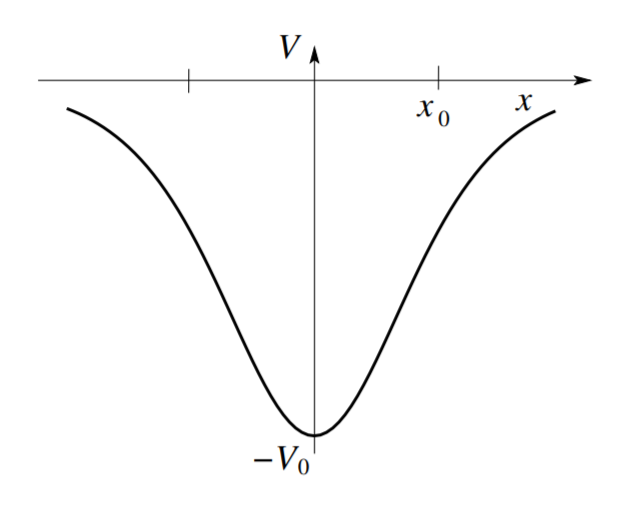
\includegraphics[scale=1]{3_35.PNG}
    \end{minipage}
    \begin{minipage}{0.5\textwidth}
        \captionsetup{font={Large}}
        \caption{The $\text{H-secant}^2$ potential $V (x) = -V_0 / cosh^2(x / x_0)$ occurs in different contexts, for example, in the treatment of the nonlinear Schrodinger equation, instantons in tunneling processes, or in the scattering of fermions.}
    \end{minipage}
\end{figure}
Here we are looking for solutions to the eigenvalue equation
%公式 3148
\begin{equation}
    \left[-\frac{\hbar^{2}}{2 m} \partial_{x}^{2}-\frac{V_{0}}{\cosh ^{2}\left(x / x_{0}\right)}-E\right] \Psi(x)=0
    \end{equation}
For $E <0$, a discrete spectrum results. We define the new one variable $y = \operatorname{tanh} (x / x_0)$ and the parameters $\alpha = \sqrt{2m | E |}/\hbar, e = \alpha x_0, k_0 = \sqrt{2mV_0} / \hbar$; then
%公式 3149
\begin{equation}
    \partial_{x} y=\frac{1 / x_{0}}{\cosh ^{2}\left(x / x_{0}\right)}, \quad \partial_{x}^{2} y=-\frac{2 / x_{0}^{2}}{\cosh ^{2}\left(x / x_{0}\right)} \tanh \frac{x}{x_{0}}
    \end{equation}
and the differential equation (3.148) for $\Psi(y)$ can be written as
%公式 3150
\begin{equation}
    \left[\underbrace{\underbrace{\partial_{y}\left[\left(1-y^{2}\right) \partial_{y}\right]+k_{0}^{2} x_{0}^{2}}_{(\mathrm{A})}-\frac{e^{2}}{1-y^{2}}}_{(B)}\right] \Psi(y)=0
    \end{equation}
The term $(A)$ can be solved with $k_0^2x_0^2 = s (s + 1)$ through the legend polynomials Ps; the complete expression $(B)$ leads to the associated Legendre polynomials. By the approach $\Psi = (1 - y^2)^{e / 2}\varphi$ we get rid of the last term,
%公式 3151
\begin{equation}
    \left(1-y^{2}\right) \partial_{y}^{2} \varphi-2(e+1) y \partial_{y} \varphi+\left[k_{0}^{2} x_{0}^{2}-e(e+1)\right] \varphi(y)=0
    \end{equation}
The transition to $\mu = (1 - y) / 2, \partial y = -\partial u / 2$, yields a hypergeometric differential equation,
%公式 3152
\begin{equation}
    [u(1-u) \partial_{u}^{2}+(e+1)(1-2 u) \partial_{u}-\underbrace{(e-s)(e+s+1)}_{e(e+1)-\underbrace{s(s+1)}_{k_{0}^{2} x_{0}^{2}}}] \varphi(u)=0
    \end{equation}
The standard form of the hypergeometric differential equation
%公式 3153
\begin{equation}
    \left\{\left[u(1-u) \partial_{u}^{2}+[\gamma-(\alpha+\beta+1) u] \partial_{u}-\alpha \beta\right\} F(\alpha, \beta, \gamma ; u)=0\right.
    \end{equation}
is going through
%公式
$$
    F(\alpha, \beta, \gamma ; u)=1+\frac{\alpha \beta}{1 ! \gamma} u+\frac{\alpha(\alpha+1)}{2 !} \frac{\beta(\beta+1)}{\gamma(\gamma+1)} u^{2}+\cdots
$$
solved. By coefficient comparison one finds the consistent set of parameters $\alpha = e - s, \beta = e + s + 1, \gamma = e + 1$, and thus the solution
%公式 3154
\begin{equation}
\begin{aligned} \varphi(u) &=F(e-s, e+s+1, e+1 ; u) \quad \text { or } \\ \Psi(y) &=\left(1-y^{2}\right)^{e / 2} F[e-s, e+s+1, e+1 ;(1-y) / 2] \end{aligned}
\end{equation}
Again, F must be a polynomial and we e
%公式 3155
\begin{equation}
\begin{aligned} e^{2} &=(s-n)^{2}=-\frac{E_{n}}{V_{0}} k_{0}^{2} x_{0}^{2} \\-E_{n} &=V_{0}\left(\frac{s-n}{x_{0} k_{0}}\right)^{2} \text { und mit } s(s+1)=k_{0}^{2} x_{0}^{2} \\ &=V_{0}\left(\frac{\sqrt{1+4 k_{0}^{2} x_{0}^{2}}-(1+2 n)}{2 x_{0} k_{0}}\right)^{2} \\ &=\frac{\hbar^{2}}{8 m x_{0}^{2}}[\sqrt{1+\frac{8 m x_{0}^{2}}{\hbar^{2}} V_{0}-(1+2 n)}]^{2} \end{aligned}
\end{equation}
Again, $n <s\backsimeq x_0k_0$ (for $s\gg 1$) and thus the number of bound states is limited; $n = 0$ is always a solution. Note that in dim = 1 every attractive potential with $V (x \to\pm\infty\to 0, V (0) <0,$ has at least one bound state. The Morse potential has $V(x\to -\infty)\to\infty$ and thus $x_0k_0 <1/2$ must be satisfied for a bound state to exist. Another nice example is the $x^{-2}$ potential in d dimensions, see Landau-Lifschitz and Phys. Rev. Lett. 85, 1590 (2000).
\section{Constant force field}
The constant force field is due to the linear potential
%公式 3156
\begin{equation}
    V(x)=-F x, \quad F>0
    \end{equation}
describe, cf. the notation in Fig. 3.36. We are looking for stationary
%图 3:36
\begin{figure}[ht]
    \begin{minipage}{0.5\textwidth}
        \centering
        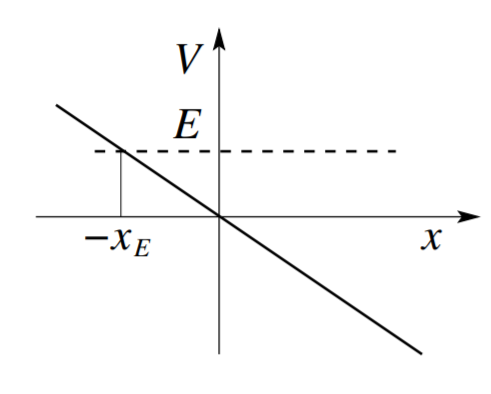
\includegraphics[scale=1]{3_36.PNG}
    \end{minipage}
    \begin{minipage}{0.5\textwidth}
        \captionsetup{font={Large}}
        \caption{The linear potential $V (x) = -F x$ describes a particle in the force field, e.g., an electron in the electric field, and is important in describing particle transport.}
    \end{minipage}
\end{figure}
Solution of the Schrodinger equation; the eigenvalue problem $H\Psi=E\Psi$ leads to the differential equation
%干 撒 3157
\begin{equation}
    \left[-\left(\hbar^{2} / 2 m\right) \partial_{x}^{2}-F x-E\right] \Psi(x)=0
    \end{equation}
with any eigenvalue $E$ as a parameter (the problem is invariant with simultaneous displacement of place and energy). As usual, we choose custom variables
%公式 3158
\begin{equation}
\begin{aligned} y &=\left(2 m F / \hbar^{2}\right)^{1 / 3}(x+E / F)=\left(x+x_{E}\right) / l_{F} \\ l_{F} &=\left(\hbar^{2} / 2 m F\right)^{1 / 3} \end{aligned}
\end{equation}
with $l_F$ of the characteristic length in the problem. The differential equation
%公式 3159
\begin{equation}
    \left(\partial_{y}^{2}+y\right) \Psi(y)=0
    \end{equation}
with the boundary condition $\Psi(y\to -\infty)\to 0$, the Airy function has $Ai (-y)$ as
Solution,
%公式 3160
\begin{equation}
    \Psi(y)=N \operatorname{Ai}(-y)=\frac{N}{\sqrt{\pi}} \int_{0}^{\infty} d \nu \cos \left(\frac{\nu^{3}}{3}-\nu y\right)
    \end{equation}
The Airy function produces the following asymptotics for $y\to\pm\infty$,
%公式 3161
\begin{equation}
\begin{array}{ll}{y \rightarrow-\infty:} & {\Psi(y) \approx \frac{N}{2|y|^{1 / 4}} e^{-\frac{2}{3}|y|^{3 / 2}} \rightarrow 0} \\ {y \rightarrow+\infty:} & {\Psi(y) \approx \frac{N}{y^{1 / 4}} \sin \left(\frac{2}{3} y^{3 / 2}+\frac{\pi}{4}\right)}\end{array}
\end{equation}
and we choose a standardization
%公式 3162
\begin{equation}
    \int_{\mathbb{R}} \Psi^{*}\left[\left(x+x_{E^{\prime}}\right) / l_{F}\right] \Psi\left[\left(x+x_{E}\right) / l_{F}\right] d x=\delta\left(E-E^{\prime}\right)
    \end{equation}
with the real wave function $\Psi^*=\Psi$. To determine the normalization factor $N$, we use the asymptotics $y\to\infty$, which gives a dominant contribution, and normalize $\Psi$ such that $\Psi\to$ yields a current density of $1 / h$ (With normalization (3.162) the wave function Ψ carries the unit $[| \Psi |^2= 1 / \text{energy · length}$ and the current density $j\sim(\hbar/2im[\Psi^*\partial_x\Psi-c.c.]$ is measured in units of $1 / \text{effect}$.), See Landau Lifschitz; as a result we find

%公式 3163
\begin{equation}
    N=1 / \sqrt{\pi F} l_{F}
    \end{equation}
With the normalization $N$ we finally find the required eigenfunction
%图 3:37
\begin{figure}[ht]
    \begin{minipage}{0.5\textwidth}
        \centering
        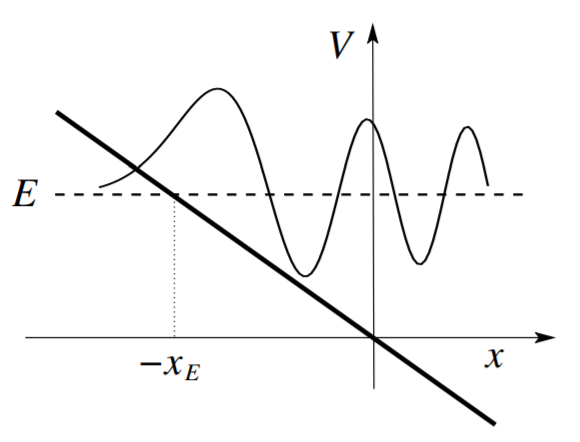
\includegraphics[scale=1]{3_37.PNG}
    \end{minipage}
    \begin{minipage}{0.5\textwidth}
        \captionsetup{font={Large}}
        \caption{Linear potential $V (x) = -F x$ with airy function as stationary solution of the associated eigenvalue problem with energy $E$.}
    \end{minipage}
\end{figure}
Ψ, cf. Fig. 3.37
%公式 3164
\begin{equation}
    \Psi(x)=\frac{1}{\sqrt{\pi F} l_{F}} \operatorname{Ai}\left(-\frac{x+E / F}{l_{F}}\right)
    \end{equation}
The function $Bi (y)$ denotes the second solution to the problem $(\partial^2_y + y) \Psi (y) = 0$ with the boundary condition $\Psi(y\to -\infty)\to\infty$; This is not normalizable and therefore unphysical.
\section{Charged particle in the electric field}
As an example of the constant force field we consider the electron with charge $q = -e <0, e> 0$ in the electric field $\vec{\varepsilon}$, see Figure 3.38 (we define the charge of the electron as $q = -e, e$ the (positive) charge unit) , Then the force $F = e\varepsilon> 0$ and write for the potential
%图 3:38
\begin{figure}[ht]
    \begin{minipage}{0.5\textwidth}
        \centering
        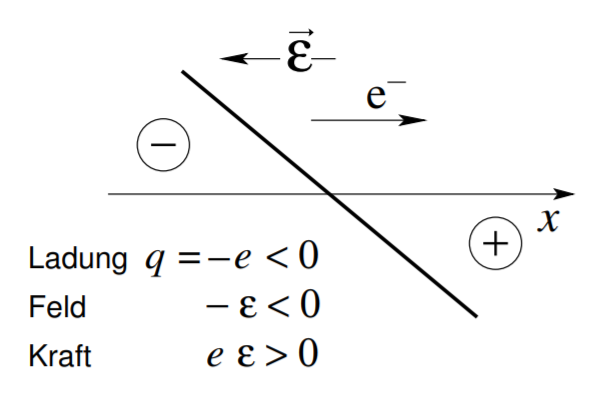
\includegraphics[scale=1]{3_38.PNG}
    \end{minipage}
    \begin{minipage}{0.5\textwidth}
        \captionsetup{font={Large}}
        \caption{Linear potential $V (x) = -e\varepsilon x$ generated by electric field $\vec{\varepsilon}$ of the power $\varepsilon$ and acting on an electronic charge $q = -e <0$. The force $F = -\partial_xV = e\varepsilon$ accelerates the particle in the positive $x$-direction.}
    \end{minipage}
\end{figure}
we $V (x) = -e\varepsilon x$. The eigenvalue problem has the known form
%公式 3165
\begin{equation}
    H \Psi_{E}=E \Psi_{E} \quad \operatorname{mit} \quad H=-\frac{\hbar^{2}}{2 m} \partial_{x}^{2}-e \mathcal{E} x
    \end{equation}
We can take the above solution and find the stationary eigenfunctions
%公式 3166
\begin{equation}
\begin{aligned} \Psi_{E}(x) &=\frac{1}{\sqrt{\pi e \mathcal{E}} l_{e \mathcal{E}}} \operatorname{Ai}\left(-\frac{x+E / e \mathcal{E}}{l_{e \mathcal{E}}}\right) \\ \Psi_{E}(x, t) &=\Psi_{E}(x) e^{-i E t / \hbar} \end{aligned}
\end{equation}
On the other hand, we can represent a constant electric field
%公式 3167
\begin{equation}
    \overrightarrow{\mathcal{E}}=-\frac{1}{c} \partial_{t} \vec{A} \Rightarrow \vec{A}=-c \overrightarrow{\mathcal{E}} t, \quad \varphi=0
    \end{equation}
The general Hamiltonian for a particle with charge
%公式 3168
\begin{equation}
    H=\frac{(\vec{p}-q \vec{A} / c)^{2}}{2 m}+q \varphi
    \end{equation}
we now choose $\varphi = 0, q = -e, \vec{A} = -c \vec{\varepsilon} t$ and get
%公式 3169
\begin{equation}
    H=\frac{(p+e \mathcal{E} t)^{2}}{2 m}=H(t)
    \end{equation}
We are looking for a solution of $i\hbar\partial_t\Psi (x, t) = H\Psi (x, t)$. With the approach
%公式 3170
\begin{equation}
    \Psi_{p}(x, t)=e^{i p x / \hbar} \varphi_{p}(t)
    \end{equation}
we receive
%公式 3171
\begin{equation}
\begin{aligned} i \hbar \partial_{t} \varphi_{p}(t) &=\frac{(p+e \mathcal{E} t)^{2}}{2 m} \varphi_{p}(t) \\ \Rightarrow \Psi_{p}(x, t) &=\exp \left[\frac{i}{\hbar}\left(p x-\int^{t} d t^{\prime} \frac{\left(p+e \mathcal{E} t^{\prime}\right)^{2}}{2 m}\right)\right] \end{aligned}
\end{equation}
The solutions $\Psi_p (x, t)$ are called Houghton functions. We compare the two solutions
%列表 对比
$$\Psi_p(x,t) \text{ Nonstationary solution to H } \text{ with }\partial_tH\neq 0. \Psi_p\sim exp[i(px-E(e)t)/\hbar] \text{ is complex and carries electricity. }\\
\Psi_E(x,t), \text{ stationary solution to H } \text{ with }\partial_tH=0. \Psi_E\sim exp[i(p(x)x-Et)/\hbar t]+c.c. p(x)x\sim \sqrt{2mFx}x\sim x^{3/2} \text{ for }x\to\infty\text{ is real, carries no electricity. }$$\\
By means of a gauge transformation we can relate the two solutions. (We apply the gauge invariance to the problem 'electron in the constant field' and start from the Hamiltonian $H (\vec{A}, t)$ in the form
%公式 3172
\begin{equation}
    H=\frac{1}{2 m}\left(\vec{p}+\frac{e}{c} \vec{A}\right)^{2}, \vec{A}=-c \overrightarrow{\mathcal{E}} t, \varphi=0
    \end{equation}
with the solutions $\Psi_p (x, t)$ of the time-dependent equation of the equation, $i\hbar\partial_t\Psi_p = H\Psi_p$. With
the conversion to $\vec{A}^{\prime} = 0 \Rightarrow \chi = -c \varepsilon tx \Rightarrow \varphi^{\prime}=\varepsilon x$ and $V (x) = -e\varphi^{\prime}= -e\varepsilon x$, we get the transformed Hamiltonian $H_{\prime} = p^2 / 2m - e\varepsilon x$ and the transformed wavefunction
%公式 3173
\begin{equation}
    \Psi_{p}^{\prime}(x, t)=\exp \left\{\frac{i}{\hbar}\left[p x-\int^{t} d t^{\prime}\left(\frac{1}{2 m}\left(p+e \mathcal{E} t^{\prime}\right)^{2}+e \mathcal{E} x\right)\right]\right\}
    \end{equation}
But is also $i \hbar\partial_t\Psi_E = H^{\prime}\Psi_E$ with $\Psi_E(x, t) = \Psi_E(x) exp (-iEt / \hbar)$. $\Psi_p^{\prime}$ and $\Psi_E$ generate complete orthogonal basis systems and can be converted into one another, for example (to check
%公式 3174
\begin{equation}
\begin{aligned} \Psi_{E}(x, 0) &=\int \frac{d p}{2 \pi \hbar} a_{E}(p) \Psi_{p}^{\prime}(x, 0) \\ a_{E}(p) &=\frac{1}{\sqrt{e \mathcal{E}}} \exp \left[-\frac{i p}{\hbar e \mathcal{E}}\left(\frac{p^{2}}{6 m}-E\right)\right] \end{aligned}
\end{equation}
)
\section{gauge transformation}
Consider a charged particle of charge q and mass m in the electromagnetic potential given by $(\varphi, \vec{A});$ the Hamiltonian in the form
%公式 3175
\begin{equation}
    H=\frac{(\vec{p}-q \vec{A} / c)^{2}}{2 m}+q \varphi
    \end{equation}
follows from the correspondence principle. The gauge transformation of the electrical potentials
%公式 3176
\begin{equation}
\begin{aligned} \vec{A} & \rightarrow \vec{A}+\nabla \chi(\vec{r}, t)=\vec{A}^{\prime} \\ \varphi & \rightarrow \varphi-\frac{1}{c} \partial_{t} \chi(\vec{r}, t)=\varphi^{\prime} \end{aligned}
\end{equation}
leave the fields $\vec{B} = \vec{\nabla} \wedge \vec{A} $ and $\vec{E}= -\vec{\nabla}\varphi - c^{-1}\partial_t\vec{A}$ and thus the Maxwell equations invariant. Here $\chi (\vec{r} , t)$ is a scalar calibration function. In quantum mechanics one also requires that the Schreiber equation is invariant, which implies a third transformation rule for the wave function,
%公式 3177
\begin{equation}
    \Psi \rightarrow \Psi \exp \left[\frac{i q}{\hbar c} \chi(\vec{r}, t)\right]=\Psi^{\prime}
    \end{equation}
the transformation (3.177) guarantees that with $i \hbar \partial_t\Psi = H (\varphi^{\prime}, \vec{A^{\prime}}, t ) \Psi^{\prime}$ also
$i \hbar \partial_t\Psi^{\prime} = H (\varphi^{\prime},\vec{A^{\prime}} t) \Psi^{\prime} $ is a solution. For the proof: Write the equation of the equation in the form $(i \hbar\partial_t - q\varphi) \Psi = (P^2 / 2m) \Psi$ with the operator $\vec{P} \equiv \vec{p} - (q / c) \vec{A}$ and show that $(i \hbar\partial_t - q\varphi^{\prime}) \Psi^{\prime} = exp (iq\chi / \hbar c) i \hbar\partial_t\Psi$ and $\vec{P^{\prime}}\Psi^{\prime} = exp (iq\chi / \hbar c) \vec{P} \Psi$ is satisfied.
